         \chapter{Electromagnetic radiation}
    \setcounter{figure}{1}
    \setcounter{subfigure}{1}
    \label{459e2bef85baf867f5850bc8338cad3a}
    
    
    
    
       
         \section{ Wave and particle nature}
    \nopagebreak
            \label{m38777} $ \hspace{-5pt}\begin{array}{cccccccccccc}   
\includegraphics[width=0.75cm]{col11305.imgs/summary_fullmarks.png} &   \end{array} $ \hspace{2 pt}\raisebox{-5 pt}{} {(section shortcode: P10050 )} \par 
    
    
    
    
    
    
  
    
    \label{m38777*cid2}
            \subsection{ Introduction}
            \nopagebreak
            
      
      \label{m38777*eip-667}Observe the things around you, your friend sitting next to you, a large tree across the field. How is it that you are able to see these things? What is it that is leaving your friend's arm and entering your eye so that you can see his arm? It is light. The light originally comes from the sun, or possibly a light bulb or burning fire. In physics, light is given the more technical term electromagnetic radiation, which includes all forms of light, not just the form which you can see with your eyes.\par \label{m38777*id186669}This chapter will focus on the electromagnetic (EM) radiation. Electromagnetic radiation is a self-propagating wave in space with electric and magnetic components. These components oscillate at right angles to each other and to the direction of propagation, and are in phase with each other. Electromagnetic radiation is classified into types according to the frequency of the wave: these types include, in order of increasing frequency, radio waves, microwaves, infrared radiation, visible light, ultraviolet radiation, X-rays and gamma rays.\par 
    
    \label{m38777*cid3}
            \subsection{ Particle/Wave Nature of Electromagnetic Radiation}
            \nopagebreak
            
      
      \label{m38777*id186686}If you watch a colony of ants walking up the wall, they look like a thin continuous black line. But as you look closer, you see that the line is made up of thousands of separated black ants.\par 
      \label{m38777*id187029}Light and all other types of electromagnetic radiation seems like a continuous wave at first, but when one performs experiments with light, one can notice that light can have both wave and particle like properties. Just like the individual ants, the light can also be made up of individual bundles of energy, or quanta of light.\par 
      \label{m38777*id187035}Light has both wave-like and particle-like properties (wave--particle duality), but only shows one or the other, depending on the kind of experiment we perform. A wave-type experiment shows the wave nature, and a particle-type experiment shows particle nature. One \textbf{cannot} test the wave and the particle nature at the same time. A particle of light is called a photon.\par 
\label{m38777*fhsst!!!underscore!!!id75}\begin{definition}
	  \begin{tabular*}{15 cm}{m{15 mm}m{}}
	\hspace*{-50pt}  
\includegraphics[width=0.5in]{col11305.imgs/psflag2.png}   & \Definition{   \label{id2452276}\textbf{ Photon }} { \label{m38777*meaningfhsst!!!underscore!!!id75}
      \label{m38777*id187051}A photon is a quantum (energy packet) of light. \par 
       } 
      \end{tabular*}
      \end{definition}

      \label{m38777*id187062}The particle nature of light can be demonstrated by the interaction of photons with matter. One way in which light interacts with matter is via the photoelectric effect, which will be studied in detail in Chapter~.\par 
\label{m38777*secfhsst!!!underscore!!!id79}
            \subsubsection{  Particle/wave nature of electromagnetic radiation }
            \nopagebreak
            
      \label{m38777*id187078}\begin{enumerate}[noitemsep, label=\textbf{\arabic*}. ] 
            \label{m38777*uid1}\item Give examples of the behaviour of EM radiation which can best be explained using a wave model.\newline
            
\label{m38777*uid2}\item Give examples of the behaviour of EM radiation which can best be explained using a particle model.\newline
            
\end{enumerate}
        
      

    
    \label{m38777*cid4}
\par \raisebox{-5 pt}{
\includegraphics[width=0.5cm]{col11305.imgs/summary_www.png}} Find the answers with the shortcodes:
 \par \begin{tabular}[h]{cccccc}
 (1.) l22  &  (2.) l2T  & \end{tabular}



            \subsection{ The wave nature of electromagnetic radiation}
            \nopagebreak
            
      
      \label{m38777*id187125}Accelerating charges emit electromagnetic waves. We have seen that a changing electric field generates a magnetic field and a changing magnetic field generates an electric field. This is the principle behind the propagation of electromagnetic waves, because electromagnetic waves, unlike sound waves, do not need a medium to travel through. EM waves propagate when an electric field oscillating in one plane produces a magnetic field oscillating in a plane at right angles to it, which produces an oscillating electric field, and so on. The propagation of electromagnetic waves can be described as \textsl{mutual induction}.\par 
      \label{m38777*id187138}These mutually regenerating fields travel through empty space at a constant speed of \begin{math}3\ensuremath{\times}{10}^{8}\phantom{\rule{0.166667em}{0ex}}\mathrm{m}\ensuremath{\cdot}{\mathrm{s}}^{-1}\end{math}, represented by \begin{math}c\end{math}.\par 
      \label{m38777*eip-43}Although an electromagnetic wave can travel through empty space, it can also travel through a medium (such as water and air). When an electromagnetic wave travels through a medium, it always travels slower than it would through empty space.\par \label{m38777*id187191}
        
    \setcounter{subfigure}{0}


	\begin{figure}[H] % horizontal\label{m38777*id187194}
    \begin{center}
    \label{m38777*id187194!!!underscore!!!media}\label{m38777*id187194!!!underscore!!!printimage}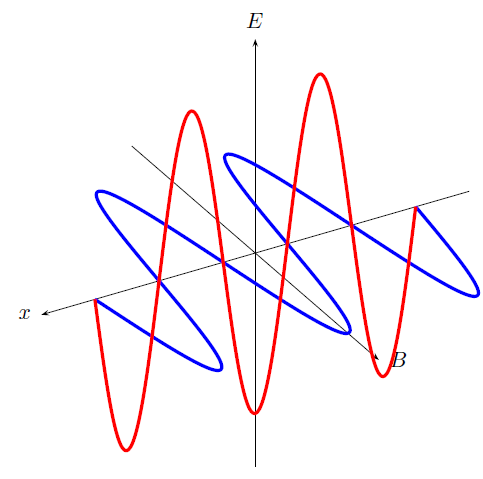
\includegraphics[width=300px]{col11305.imgs/m38777_PG12C15_001.png} % m38777;PG12C15\_001.png;;;6.0;8.5;
        
      \vspace{2pt}
    \vspace{.1in}
    
    \end{center}

 \end{figure}   

    \addtocounter{footnote}{-0}
    
      \par \label{m38777*eip-808}Since an electromagnetic wave is still a wave, the following equation still applies:\par \label{m38777*eip-181}\nopagebreak\noindent{}\settowidth{\mymathboxwidth}{\begin{equation}
    v=f\ensuremath{\cdot}\lambda \tag{10.1}
      \end{equation}
    }
    \typeout{Columnwidth = \the\columnwidth}\typeout{math as usual width = \the\mymathboxwidth}
    \ifthenelse{\lengthtest{\mymathboxwidth < \columnwidth}}{% if the math fits, do it again, for real
    \begin{equation}
    v=f\ensuremath{\cdot}\lambda \tag{10.1}
      \end{equation}
    }{% else, if it doesn't fit
    \setlength{\mymathboxwidth}{\columnwidth}
      \addtolength{\mymathboxwidth}{-48pt}
    \par\vspace{12pt}\noindent\begin{minipage}{\columnwidth}
    \parbox[t]{\mymathboxwidth}{\large\begin{math}
    v=f\ensuremath{\cdot}\lambda \end{math}}\hfill
    \parbox[t]{48pt}{\raggedleft 
    (10.1)}
    \end{minipage}\vspace{12pt}\par
    }% end of conditional for this bit of math
    \typeout{math as usual width = \the\mymathboxwidth}
    
      \label{m38777*eip-601}Except that we can replace \begin{math}v\end{math} with \begin{math}c\end{math} (if we're dealing with an electromagnetic wave travelling through empty space):\par \label{m38777*eip-194}\nopagebreak\noindent{}\settowidth{\mymathboxwidth}{\begin{equation}
    c=f\ensuremath{\cdot}\lambda \tag{10.2}
      \end{equation}
    }
    \typeout{Columnwidth = \the\columnwidth}\typeout{math as usual width = \the\mymathboxwidth}
    \ifthenelse{\lengthtest{\mymathboxwidth < \columnwidth}}{% if the math fits, do it again, for real
    \begin{equation}
    c=f\ensuremath{\cdot}\lambda \tag{10.2}
      \end{equation}
    }{% else, if it doesn't fit
    \setlength{\mymathboxwidth}{\columnwidth}
      \addtolength{\mymathboxwidth}{-48pt}
    \par\vspace{12pt}\noindent\begin{minipage}{\columnwidth}
    \parbox[t]{\mymathboxwidth}{\large\begin{math}
    c=f\ensuremath{\cdot}\lambda \end{math}}\hfill
    \parbox[t]{48pt}{\raggedleft 
    (10.2)}
    \end{minipage}\vspace{12pt}\par
    }% end of conditional for this bit of math
    \typeout{math as usual width = \the\mymathboxwidth}
    
      \par
            \label{m38777*eip-923}\vspace{.5cm} 
      
      \noindent
      \hspace*{-30pt}
\includegraphics[width=0.5in]{col11305.imgs/pspencil2.png}   \raisebox{25mm}{   
      \begin{mdframed}[linewidth=4, leftmargin=40, rightmargin=40]  
      \begin{exercise}
    \noindent\textbf{Exercise 10.1: EM radiation I}\label{m38777*probfhsst!!!underscore!!!id246}
      \label{m38777*id187899}Calculate the frequency of an electromagnetic wave with a wavelength of \begin{math}4,2\ensuremath{\times}{10}^{-7}\end{math} m \par 
      \vspace{5pt}
      \label{m38777*solfhsst!!!underscore!!!id249}\noindent\textbf{Solution to Exercise } \label{m38777*listfhsst!!!underscore!!!id249}\begin{enumerate}[noitemsep, label=\textbf{Step} \textbf{\arabic*}. ] 
            \leftskip=20pt\rightskip=\leftskip\item  
      \label{m38777*id187948}We use the formula: \begin{math}c=f\lambda \end{math} to calculate frequency. The speed of light is a constant \begin{math}3\ensuremath{\times}{10}^{8}\end{math}m/s.\par 
      \label{m38777*id187985}\nopagebreak\noindent{}
        \settowidth{\mymathboxwidth}{\begin{equation}
    \begin{array}{ccc}\hfill c& =& f\lambda \hfill \\ \hfill 3\ensuremath{\times}{10}^{8}& =& f\ensuremath{\times}4,2\ensuremath{\times}{10}^{-7}\hfill \\ \hfill f& =& 7,14\ensuremath{\times}{10}^{14}\mathrm{Hz}\hfill \end{array}\tag{10.3}
      \end{equation}
    }
    \typeout{Columnwidth = \the\columnwidth}\typeout{math as usual width = \the\mymathboxwidth}
    \ifthenelse{\lengthtest{\mymathboxwidth < \columnwidth}}{% if the math fits, do it again, for real
    \begin{equation}
    \begin{array}{ccc}\hfill c& =& f\lambda \hfill \\ \hfill 3\ensuremath{\times}{10}^{8}& =& f\ensuremath{\times}4,2\ensuremath{\times}{10}^{-7}\hfill \\ \hfill f& =& 7,14\ensuremath{\times}{10}^{14}\mathrm{Hz}\hfill \end{array}\tag{10.3}
      \end{equation}
    }{% else, if it doesn't fit
    \setlength{\mymathboxwidth}{\columnwidth}
      \addtolength{\mymathboxwidth}{-48pt}
    \par\vspace{12pt}\noindent\begin{minipage}{\columnwidth}
    \parbox[t]{\mymathboxwidth}{\large\begin{math}
    c=f\lambda 3\ensuremath{\times}{10}^{8}=f\ensuremath{\times}4,2\ensuremath{\times}{10}^{-7}f=7,14\ensuremath{\times}{10}^{14}\mathrm{Hz}\end{math}}\hfill
    \parbox[t]{48pt}{\raggedleft 
    (10.3)}
    \end{minipage}\vspace{12pt}\par
    }% end of conditional for this bit of math
    \typeout{math as usual width = \the\mymathboxwidth}
    
      
      
      \end{enumerate}
         

    \end{exercise}
    \end{mdframed}
    }
    \noindent
  \par
            \label{m38777*eip-696}\vspace{.5cm} 
      
      \noindent
      \hspace*{-30pt}
\includegraphics[width=0.5in]{col11305.imgs/pspencil2.png}   \raisebox{25mm}{   
      \begin{mdframed}[linewidth=4, leftmargin=40, rightmargin=40]  
      \begin{exercise}
    \noindent\textbf{Exercise 10.2: EM Radiation II}\label{m38777*probfhsst!!!underscore!!!id329}
      \label{m38777*id188123}An electromagnetic wave has a wavelength of \begin{math}200\phantom{\rule{3.33333pt}{0ex}}\mathrm{nm}\end{math}. What is the frequency of the radiation? \par 
      \vspace{5pt}
      \label{m38777*solfhsst!!!underscore!!!id332}\noindent\textbf{Solution to Exercise } \label{m38777*listfhsst!!!underscore!!!id332}\begin{enumerate}[noitemsep, label=\textbf{Step} \textbf{\arabic*}. ] 
            \leftskip=20pt\rightskip=\leftskip\item  
      \label{m38777*id188341}Recall that all radiation travels at the speed of light (\begin{math}c\end{math}) in vacuum.
Since the question does not specify through what type of material the wave
is traveling, one can assume that it is traveling through a vacuum.
We can identify two properties of the radiation - \begin{math}wavelength\phantom{\rule{3.33333pt}{0ex}}\left(200\phantom{\rule{3.33333pt}{0ex}}\mathrm{nm}\right)\end{math} and speed (\begin{math}c\end{math}).\par 
      \item  
      \label{m38777*id188424}\nopagebreak\noindent{}
        \settowidth{\mymathboxwidth}{\begin{equation}
    \begin{array}{ccc}\hfill c& =& f\lambda \hfill \\ \hfill 3\ensuremath{\times}{10}^{8}& =& f\ensuremath{\times}200\ensuremath{\times}{10}^{-9}\hfill \\ \hfill f& =& 1.5\ensuremath{\times}{10}^{15}\phantom{\rule{4pt}{0ex}}\mathrm{Hz}\hfill \end{array}\tag{10.4}
      \end{equation}
    }
    \typeout{Columnwidth = \the\columnwidth}\typeout{math as usual width = \the\mymathboxwidth}
    \ifthenelse{\lengthtest{\mymathboxwidth < \columnwidth}}{% if the math fits, do it again, for real
    \begin{equation}
    \begin{array}{ccc}\hfill c& =& f\lambda \hfill \\ \hfill 3\ensuremath{\times}{10}^{8}& =& f\ensuremath{\times}200\ensuremath{\times}{10}^{-9}\hfill \\ \hfill f& =& 1.5\ensuremath{\times}{10}^{15}\phantom{\rule{4pt}{0ex}}\mathrm{Hz}\hfill \end{array}\tag{10.4}
      \end{equation}
    }{% else, if it doesn't fit
    \setlength{\mymathboxwidth}{\columnwidth}
      \addtolength{\mymathboxwidth}{-48pt}
    \par\vspace{12pt}\noindent\begin{minipage}{\columnwidth}
    \parbox[t]{\mymathboxwidth}{\large\begin{math}
    c=f\lambda 3\ensuremath{\times}{10}^{8}=f\ensuremath{\times}200\ensuremath{\times}{10}^{-9}f=1.5\ensuremath{\times}{10}^{15}\phantom{\rule{4pt}{0ex}}\mathrm{Hz}\end{math}}\hfill
    \parbox[t]{48pt}{\raggedleft 
    (10.4)}
    \end{minipage}\vspace{12pt}\par
    }% end of conditional for this bit of math
    \typeout{math as usual width = \the\mymathboxwidth}
    
      
      
      \end{enumerate}
         

    \end{exercise}
    \end{mdframed}
    }
    \noindent
  
    

  \label{m38777**end}
          
         \section{ Electromagnetic spectrum}
    \nopagebreak
            \label{m38778} $ \hspace{-5pt}\begin{array}{cccccccccccc}   
\includegraphics[width=0.75cm]{col11305.imgs/summary_fullmarks.png} &   \end{array} $ \hspace{2 pt}\raisebox{-5 pt}{} {(section shortcode: P10051 )} \par 
    
    
    
    
    
    
  
    \label{m38778*cid5}
            \subsection{ Electromagnetic spectrum}
            \nopagebreak
            
      
      
    \setcounter{subfigure}{0}


	\begin{figure}[H] % horizontal\label{m38778*uid3}
    \begin{center}
    \rule[.1in]{\figurerulewidth}{.005in} \\
        \label{m38778*uid3!!!underscore!!!media}\label{m38778*uid3!!!underscore!!!printimage}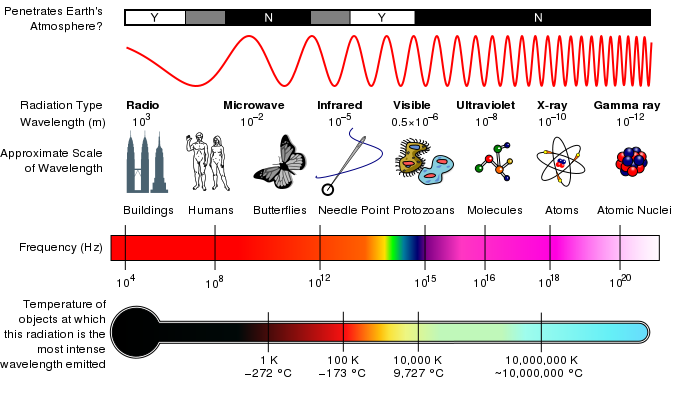
\includegraphics[width=\columnwidth]{col11305.imgs/m38778_EM_Spectrum_Properties_edit.png} % m38778;EM\_Spectrum\_Properties\_edit.png;;;6.0;8.5;
        
      \vspace{2pt}
    \vspace{\rubberspace}\par \begin{cnxcaption}
	  \small \textbf{Figure 10.2: }The electromagnetic spectrum as a function of frequency. The different types according to wavelength are shown as well as everyday comparisons.
	\end{cnxcaption}
      
    \vspace{.1in}
    \rule[.1in]{\figurerulewidth}{.005in} \\
        
    \end{center}

 \end{figure}   

    \addtocounter{footnote}{-0}
    
      
      \label{m38778*id187230}Electromagnetic radiation allows us to observe the world around us. Some materials and objects emit electromagnetic radiation and some reflect the electromagnetic radiation emitted by other objects (such as the Sun, a light bulb or a fire). When electromagnetic radiation comes from an object (whether the radiation is emitted or reflected by the object) and enters the eye, we see that object. Everything you see around you either emits or reflects electromagnetic radiation or both.\par 

      \label{m38778*eip-532}Electromagnetic radiation comes in a wide range of frequencies (or wavelengths) and the frequencies of radiation the human eye is sensitive to is only a very small part of it. The collection of all possible frequencies of electromagnetic radiation is called the electromagnetic spectrum, which (for convenience) is divided into sections (such as radio, microwave, infrared, visible, ultraviolet, X-rays and gamma-rays).\par \label{m38778*eip-855}The electromagnetic spectrum is continuous (has no gaps) and infinite. In practice, we can only use electromagnetic radiation with wavelengths between (very roughly) \begin{math}{10}^{-14}\mathrm{m}\end{math} (very high energy gamma rays) and \begin{math}{10}^{15}\mathrm{m}\end{math} (very long wavelength radio waves) due to technological limitations in the detectors used to receive electromagnetic radiation and in the devices used to produce or emit electromagnetic radiation.\par \label{m38778*id187253}The various frequencies (or wavelengths) of electromagnetic radiation coming from a particular object or material depends on how the object or material reflects and/or emits electromagnetic radiation.\par 
\label{m38778*secfhsst!!!underscore!!!id117}
            \subsubsection{  Wave Nature of EM Radiation }
            \nopagebreak
            
      \label{m38778*id187264}\begin{enumerate}[noitemsep, label=\textbf{\arabic*}. ] 
            \label{m38778*uid4}\item List one source of electromagnetic waves. Hint: consider the spectrum diagram and look at the names we give to different wavelengths.\newline
            
\label{m38778*uid5}\item Explain how an EM wave propagates, with the aid of a diagram.\newline
            
\label{m38778*uid6}\item What is the speed of light? What symbol is used to refer to the speed of light? Does the speed of light change?\newline
            
\label{m38778*uid7}\item Do EM waves need a medium to travel through?\newline
            
\end{enumerate}
        
      

      
      \label{m38778*id187332}Table 10.1 lists the wavelength- and frequency ranges of the divisions of the electromagnetic spectrum.\par 
      
    % \textbf{m38778*uid8}\par
    
    % how many colspecs?  3
          % name: cnx:colspec
            % colnum: 1
            % colwidth: 10*
            % latex-name: columna
            % colname: 
            % align/tgroup-align/default: //left
            % -------------------------
            % name: cnx:colspec
            % colnum: 2
            % colwidth: 10*
            % latex-name: columnb
            % colname: 
            % align/tgroup-align/default: //left
            % -------------------------
            % name: cnx:colspec
            % colnum: 3
            % colwidth: 10*
            % latex-name: columnc
            % colname: 
            % align/tgroup-align/default: //left
            % -------------------------
      
    
    \setlength\mytablespace{6\tabcolsep}
    \addtolength\mytablespace{4\arrayrulewidth}
    \setlength\mytablewidth{\linewidth}
        
    
    \setlength\mytableroom{\mytablewidth}
    \addtolength\mytableroom{-\mytablespace}
    
    \setlength\myfixedwidth{0pt}
    \setlength\mystarwidth{\mytableroom}
        \addtolength\mystarwidth{-\myfixedwidth}
        \divide\mystarwidth 30
        
    
      % ----- Begin capturing width of table in LR mode woof
      \settowidth{\mytableboxwidth}{\begin{tabular}[t]{|l|l|l|}\hline
    % count in rowspan-info-nodeset: 3
    % align/colidx: left,1
    
    % rowcount: '0' | start: 'false' | colidx: '1'
    
        % Formatting a regular cell and recurring on the next sibling
        
                \textbf{Category}
               &
      % align/colidx: left,2
    
    % rowcount: '0' | start: 'false' | colidx: '2'
    
        % Formatting a regular cell and recurring on the next sibling
        
                \textbf{Range of Wavelengths (nm)}
               &
      % align/colidx: left,3
    
    % rowcount: '0' | start: 'false' | colidx: '3'
    
        % Formatting a regular cell and recurring on the next sibling
        
                \textbf{Range of Frequencies (Hz)}
              % make-rowspan-placeholders
    % rowspan info: col1 '0' | 'false' | '' || col2 '0' | 'false' | '' || col3 '0' | 'false' | ''
     \tabularnewline\cline{1-1}\cline{2-2}\cline{3-3}
      %--------------------------------------------------------------------
    % align/colidx: left,1
    
    % rowcount: '0' | start: 'false' | colidx: '1'
    
        % Formatting a regular cell and recurring on the next sibling
        gamma rays &
      % align/colidx: left,2
    
    % rowcount: '0' | start: 'false' | colidx: '2'
    
        % Formatting a regular cell and recurring on the next sibling
        \begin{math}\lessthan{}\end{math}1 &
      % align/colidx: left,3
    
    % rowcount: '0' | start: 'false' | colidx: '3'
    
        % Formatting a regular cell and recurring on the next sibling
        
                \begin{math}\greatthan{}3\ensuremath{\times}{10}^{19}\end{math}
              % make-rowspan-placeholders
    % rowspan info: col1 '0' | 'false' | '' || col2 '0' | 'false' | '' || col3 '0' | 'false' | ''
     \tabularnewline\cline{1-1}\cline{2-2}\cline{3-3}
      %--------------------------------------------------------------------
    % align/colidx: left,1
    
    % rowcount: '0' | start: 'false' | colidx: '1'
    
        % Formatting a regular cell and recurring on the next sibling
        X-rays &
      % align/colidx: left,2
    
    % rowcount: '0' | start: 'false' | colidx: '2'
    
        % Formatting a regular cell and recurring on the next sibling
        1-10 &
      % align/colidx: left,3
    
    % rowcount: '0' | start: 'false' | colidx: '3'
    
        % Formatting a regular cell and recurring on the next sibling
        \begin{math}3\ensuremath{\times}{10}^{17}\end{math}-\begin{math}3\ensuremath{\times}{10}^{19}\end{math}% make-rowspan-placeholders
    % rowspan info: col1 '0' | 'false' | '' || col2 '0' | 'false' | '' || col3 '0' | 'false' | ''
     \tabularnewline\cline{1-1}\cline{2-2}\cline{3-3}
      %--------------------------------------------------------------------
    % align/colidx: left,1
    
    % rowcount: '0' | start: 'false' | colidx: '1'
    
        % Formatting a regular cell and recurring on the next sibling
        ultraviolet light &
      % align/colidx: left,2
    
    % rowcount: '0' | start: 'false' | colidx: '2'
    
        % Formatting a regular cell and recurring on the next sibling
        10-400 &
      % align/colidx: left,3
    
    % rowcount: '0' | start: 'false' | colidx: '3'
    
        % Formatting a regular cell and recurring on the next sibling
        \begin{math}7,5\ensuremath{\times}{10}^{14}\end{math}-\begin{math}3\ensuremath{\times}{10}^{17}\end{math}% make-rowspan-placeholders
    % rowspan info: col1 '0' | 'false' | '' || col2 '0' | 'false' | '' || col3 '0' | 'false' | ''
     \tabularnewline\cline{1-1}\cline{2-2}\cline{3-3}
      %--------------------------------------------------------------------
    % align/colidx: left,1
    
    % rowcount: '0' | start: 'false' | colidx: '1'
    
        % Formatting a regular cell and recurring on the next sibling
        visible light &
      % align/colidx: left,2
    
    % rowcount: '0' | start: 'false' | colidx: '2'
    
        % Formatting a regular cell and recurring on the next sibling
        400-700 &
      % align/colidx: left,3
    
    % rowcount: '0' | start: 'false' | colidx: '3'
    
        % Formatting a regular cell and recurring on the next sibling
        \begin{math}4,3\ensuremath{\times}{10}^{14}\end{math}-\begin{math}7,5\ensuremath{\times}{10}^{14}\end{math}% make-rowspan-placeholders
    % rowspan info: col1 '0' | 'false' | '' || col2 '0' | 'false' | '' || col3 '0' | 'false' | ''
     \tabularnewline\cline{1-1}\cline{2-2}\cline{3-3}
      %--------------------------------------------------------------------
    % align/colidx: left,1
    
    % rowcount: '0' | start: 'false' | colidx: '1'
    
        % Formatting a regular cell and recurring on the next sibling
        infrared &
      % align/colidx: left,2
    
    % rowcount: '0' | start: 'false' | colidx: '2'
    
        % Formatting a regular cell and recurring on the next sibling
        700-\begin{math}{10}^{5}\end{math} &
      % align/colidx: left,3
    
    % rowcount: '0' | start: 'false' | colidx: '3'
    
        % Formatting a regular cell and recurring on the next sibling
        \begin{math}3\ensuremath{\times}{10}^{12}\end{math}-\begin{math}4,3\ensuremath{\times}{10}^{19}\end{math}% make-rowspan-placeholders
    % rowspan info: col1 '0' | 'false' | '' || col2 '0' | 'false' | '' || col3 '0' | 'false' | ''
     \tabularnewline\cline{1-1}\cline{2-2}\cline{3-3}
      %--------------------------------------------------------------------
    % align/colidx: left,1
    
    % rowcount: '0' | start: 'false' | colidx: '1'
    
        % Formatting a regular cell and recurring on the next sibling
        microwave &
      % align/colidx: left,2
    
    % rowcount: '0' | start: 'false' | colidx: '2'
    
        % Formatting a regular cell and recurring on the next sibling
        
                \begin{math}{10}^{5}-{10}^{8}\end{math}
               &
      % align/colidx: left,3
    
    % rowcount: '0' | start: 'false' | colidx: '3'
    
        % Formatting a regular cell and recurring on the next sibling
        \begin{math}3\ensuremath{\times}{10}^{9}\end{math}-\begin{math}3\ensuremath{\times}{10}^{12}\end{math}% make-rowspan-placeholders
    % rowspan info: col1 '0' | 'false' | '' || col2 '0' | 'false' | '' || col3 '0' | 'false' | ''
     \tabularnewline\cline{1-1}\cline{2-2}\cline{3-3}
      %--------------------------------------------------------------------
    % align/colidx: left,1
    
    % rowcount: '0' | start: 'false' | colidx: '1'
    
        % Formatting a regular cell and recurring on the next sibling
        radio waves &
      % align/colidx: left,2
    
    % rowcount: '0' | start: 'false' | colidx: '2'
    
        % Formatting a regular cell and recurring on the next sibling
        
                \begin{math}\greatthan{}{10}^{8}\end{math}
               &
      % align/colidx: left,3
    
    % rowcount: '0' | start: 'false' | colidx: '3'
    
        % Formatting a regular cell and recurring on the next sibling
        
                \begin{math}\lessthan{}3\ensuremath{\times}{10}^{9}\end{math}
              % make-rowspan-placeholders
    % rowspan info: col1 '0' | 'false' | '' || col2 '0' | 'false' | '' || col3 '0' | 'false' | ''
     \tabularnewline\cline{1-1}\cline{2-2}\cline{3-3}
      %--------------------------------------------------------------------
    \end{tabular}} % end mytableboxwidth set
      \addtocounter{footnote}{-0}
      
      % ----- End capturing width of table in LR mode
    
        % ----- LR or paragraph mode: must test
        % ----- Begin capturing height of table
        \settoheight{\mytableboxheight}{\begin{tabular}[t]{|l|l|l|}\hline
    % count in rowspan-info-nodeset: 3
    % align/colidx: left,1
    
    % rowcount: '0' | start: 'false' | colidx: '1'
    
        % Formatting a regular cell and recurring on the next sibling
        
                \textbf{Category}
               &
      % align/colidx: left,2
    
    % rowcount: '0' | start: 'false' | colidx: '2'
    
        % Formatting a regular cell and recurring on the next sibling
        
                \textbf{Range of Wavelengths (nm)}
               &
      % align/colidx: left,3
    
    % rowcount: '0' | start: 'false' | colidx: '3'
    
        % Formatting a regular cell and recurring on the next sibling
        
                \textbf{Range of Frequencies (Hz)}
              % make-rowspan-placeholders
    % rowspan info: col1 '0' | 'false' | '' || col2 '0' | 'false' | '' || col3 '0' | 'false' | ''
     \tabularnewline\cline{1-1}\cline{2-2}\cline{3-3}
      %--------------------------------------------------------------------
    % align/colidx: left,1
    
    % rowcount: '0' | start: 'false' | colidx: '1'
    
        % Formatting a regular cell and recurring on the next sibling
        gamma rays &
      % align/colidx: left,2
    
    % rowcount: '0' | start: 'false' | colidx: '2'
    
        % Formatting a regular cell and recurring on the next sibling
        \begin{math}\lessthan{}\end{math}1 &
      % align/colidx: left,3
    
    % rowcount: '0' | start: 'false' | colidx: '3'
    
        % Formatting a regular cell and recurring on the next sibling
        
                \begin{math}\greatthan{}3\ensuremath{\times}{10}^{19}\end{math}
              % make-rowspan-placeholders
    % rowspan info: col1 '0' | 'false' | '' || col2 '0' | 'false' | '' || col3 '0' | 'false' | ''
     \tabularnewline\cline{1-1}\cline{2-2}\cline{3-3}
      %--------------------------------------------------------------------
    % align/colidx: left,1
    
    % rowcount: '0' | start: 'false' | colidx: '1'
    
        % Formatting a regular cell and recurring on the next sibling
        X-rays &
      % align/colidx: left,2
    
    % rowcount: '0' | start: 'false' | colidx: '2'
    
        % Formatting a regular cell and recurring on the next sibling
        1-10 &
      % align/colidx: left,3
    
    % rowcount: '0' | start: 'false' | colidx: '3'
    
        % Formatting a regular cell and recurring on the next sibling
        \begin{math}3\ensuremath{\times}{10}^{17}\end{math}-\begin{math}3\ensuremath{\times}{10}^{19}\end{math}% make-rowspan-placeholders
    % rowspan info: col1 '0' | 'false' | '' || col2 '0' | 'false' | '' || col3 '0' | 'false' | ''
     \tabularnewline\cline{1-1}\cline{2-2}\cline{3-3}
      %--------------------------------------------------------------------
    % align/colidx: left,1
    
    % rowcount: '0' | start: 'false' | colidx: '1'
    
        % Formatting a regular cell and recurring on the next sibling
        ultraviolet light &
      % align/colidx: left,2
    
    % rowcount: '0' | start: 'false' | colidx: '2'
    
        % Formatting a regular cell and recurring on the next sibling
        10-400 &
      % align/colidx: left,3
    
    % rowcount: '0' | start: 'false' | colidx: '3'
    
        % Formatting a regular cell and recurring on the next sibling
        \begin{math}7,5\ensuremath{\times}{10}^{14}\end{math}-\begin{math}3\ensuremath{\times}{10}^{17}\end{math}% make-rowspan-placeholders
    % rowspan info: col1 '0' | 'false' | '' || col2 '0' | 'false' | '' || col3 '0' | 'false' | ''
     \tabularnewline\cline{1-1}\cline{2-2}\cline{3-3}
      %--------------------------------------------------------------------
    % align/colidx: left,1
    
    % rowcount: '0' | start: 'false' | colidx: '1'
    
        % Formatting a regular cell and recurring on the next sibling
        visible light &
      % align/colidx: left,2
    
    % rowcount: '0' | start: 'false' | colidx: '2'
    
        % Formatting a regular cell and recurring on the next sibling
        400-700 &
      % align/colidx: left,3
    
    % rowcount: '0' | start: 'false' | colidx: '3'
    
        % Formatting a regular cell and recurring on the next sibling
        \begin{math}4,3\ensuremath{\times}{10}^{14}\end{math}-\begin{math}7,5\ensuremath{\times}{10}^{14}\end{math}% make-rowspan-placeholders
    % rowspan info: col1 '0' | 'false' | '' || col2 '0' | 'false' | '' || col3 '0' | 'false' | ''
     \tabularnewline\cline{1-1}\cline{2-2}\cline{3-3}
      %--------------------------------------------------------------------
    % align/colidx: left,1
    
    % rowcount: '0' | start: 'false' | colidx: '1'
    
        % Formatting a regular cell and recurring on the next sibling
        infrared &
      % align/colidx: left,2
    
    % rowcount: '0' | start: 'false' | colidx: '2'
    
        % Formatting a regular cell and recurring on the next sibling
        700-\begin{math}{10}^{5}\end{math} &
      % align/colidx: left,3
    
    % rowcount: '0' | start: 'false' | colidx: '3'
    
        % Formatting a regular cell and recurring on the next sibling
        \begin{math}3\ensuremath{\times}{10}^{12}\end{math}-\begin{math}4,3\ensuremath{\times}{10}^{19}\end{math}% make-rowspan-placeholders
    % rowspan info: col1 '0' | 'false' | '' || col2 '0' | 'false' | '' || col3 '0' | 'false' | ''
     \tabularnewline\cline{1-1}\cline{2-2}\cline{3-3}
      %--------------------------------------------------------------------
    % align/colidx: left,1
    
    % rowcount: '0' | start: 'false' | colidx: '1'
    
        % Formatting a regular cell and recurring on the next sibling
        microwave &
      % align/colidx: left,2
    
    % rowcount: '0' | start: 'false' | colidx: '2'
    
        % Formatting a regular cell and recurring on the next sibling
        
                \begin{math}{10}^{5}-{10}^{8}\end{math}
               &
      % align/colidx: left,3
    
    % rowcount: '0' | start: 'false' | colidx: '3'
    
        % Formatting a regular cell and recurring on the next sibling
        \begin{math}3\ensuremath{\times}{10}^{9}\end{math}-\begin{math}3\ensuremath{\times}{10}^{12}\end{math}% make-rowspan-placeholders
    % rowspan info: col1 '0' | 'false' | '' || col2 '0' | 'false' | '' || col3 '0' | 'false' | ''
     \tabularnewline\cline{1-1}\cline{2-2}\cline{3-3}
      %--------------------------------------------------------------------
    % align/colidx: left,1
    
    % rowcount: '0' | start: 'false' | colidx: '1'
    
        % Formatting a regular cell and recurring on the next sibling
        radio waves &
      % align/colidx: left,2
    
    % rowcount: '0' | start: 'false' | colidx: '2'
    
        % Formatting a regular cell and recurring on the next sibling
        
                \begin{math}\greatthan{}{10}^{8}\end{math}
               &
      % align/colidx: left,3
    
    % rowcount: '0' | start: 'false' | colidx: '3'
    
        % Formatting a regular cell and recurring on the next sibling
        
                \begin{math}\lessthan{}3\ensuremath{\times}{10}^{9}\end{math}
              % make-rowspan-placeholders
    % rowspan info: col1 '0' | 'false' | '' || col2 '0' | 'false' | '' || col3 '0' | 'false' | ''
     \tabularnewline\cline{1-1}\cline{2-2}\cline{3-3}
      %--------------------------------------------------------------------
    \end{tabular}} % end mytableboxheight set
        \settodepth{\mytableboxdepth}{\begin{tabular}[t]{|l|l|l|}\hline
    % count in rowspan-info-nodeset: 3
    % align/colidx: left,1
    
    % rowcount: '0' | start: 'false' | colidx: '1'
    
        % Formatting a regular cell and recurring on the next sibling
        
                \textbf{Category}
               &
      % align/colidx: left,2
    
    % rowcount: '0' | start: 'false' | colidx: '2'
    
        % Formatting a regular cell and recurring on the next sibling
        
                \textbf{Range of Wavelengths (nm)}
               &
      % align/colidx: left,3
    
    % rowcount: '0' | start: 'false' | colidx: '3'
    
        % Formatting a regular cell and recurring on the next sibling
        
                \textbf{Range of Frequencies (Hz)}
              % make-rowspan-placeholders
    % rowspan info: col1 '0' | 'false' | '' || col2 '0' | 'false' | '' || col3 '0' | 'false' | ''
     \tabularnewline\cline{1-1}\cline{2-2}\cline{3-3}
      %--------------------------------------------------------------------
    % align/colidx: left,1
    
    % rowcount: '0' | start: 'false' | colidx: '1'
    
        % Formatting a regular cell and recurring on the next sibling
        gamma rays &
      % align/colidx: left,2
    
    % rowcount: '0' | start: 'false' | colidx: '2'
    
        % Formatting a regular cell and recurring on the next sibling
        \begin{math}\lessthan{}\end{math}1 &
      % align/colidx: left,3
    
    % rowcount: '0' | start: 'false' | colidx: '3'
    
        % Formatting a regular cell and recurring on the next sibling
        
                \begin{math}\greatthan{}3\ensuremath{\times}{10}^{19}\end{math}
              % make-rowspan-placeholders
    % rowspan info: col1 '0' | 'false' | '' || col2 '0' | 'false' | '' || col3 '0' | 'false' | ''
     \tabularnewline\cline{1-1}\cline{2-2}\cline{3-3}
      %--------------------------------------------------------------------
    % align/colidx: left,1
    
    % rowcount: '0' | start: 'false' | colidx: '1'
    
        % Formatting a regular cell and recurring on the next sibling
        X-rays &
      % align/colidx: left,2
    
    % rowcount: '0' | start: 'false' | colidx: '2'
    
        % Formatting a regular cell and recurring on the next sibling
        1-10 &
      % align/colidx: left,3
    
    % rowcount: '0' | start: 'false' | colidx: '3'
    
        % Formatting a regular cell and recurring on the next sibling
        \begin{math}3\ensuremath{\times}{10}^{17}\end{math}-\begin{math}3\ensuremath{\times}{10}^{19}\end{math}% make-rowspan-placeholders
    % rowspan info: col1 '0' | 'false' | '' || col2 '0' | 'false' | '' || col3 '0' | 'false' | ''
     \tabularnewline\cline{1-1}\cline{2-2}\cline{3-3}
      %--------------------------------------------------------------------
    % align/colidx: left,1
    
    % rowcount: '0' | start: 'false' | colidx: '1'
    
        % Formatting a regular cell and recurring on the next sibling
        ultraviolet light &
      % align/colidx: left,2
    
    % rowcount: '0' | start: 'false' | colidx: '2'
    
        % Formatting a regular cell and recurring on the next sibling
        10-400 &
      % align/colidx: left,3
    
    % rowcount: '0' | start: 'false' | colidx: '3'
    
        % Formatting a regular cell and recurring on the next sibling
        \begin{math}7,5\ensuremath{\times}{10}^{14}\end{math}-\begin{math}3\ensuremath{\times}{10}^{17}\end{math}% make-rowspan-placeholders
    % rowspan info: col1 '0' | 'false' | '' || col2 '0' | 'false' | '' || col3 '0' | 'false' | ''
     \tabularnewline\cline{1-1}\cline{2-2}\cline{3-3}
      %--------------------------------------------------------------------
    % align/colidx: left,1
    
    % rowcount: '0' | start: 'false' | colidx: '1'
    
        % Formatting a regular cell and recurring on the next sibling
        visible light &
      % align/colidx: left,2
    
    % rowcount: '0' | start: 'false' | colidx: '2'
    
        % Formatting a regular cell and recurring on the next sibling
        400-700 &
      % align/colidx: left,3
    
    % rowcount: '0' | start: 'false' | colidx: '3'
    
        % Formatting a regular cell and recurring on the next sibling
        \begin{math}4,3\ensuremath{\times}{10}^{14}\end{math}-\begin{math}7,5\ensuremath{\times}{10}^{14}\end{math}% make-rowspan-placeholders
    % rowspan info: col1 '0' | 'false' | '' || col2 '0' | 'false' | '' || col3 '0' | 'false' | ''
     \tabularnewline\cline{1-1}\cline{2-2}\cline{3-3}
      %--------------------------------------------------------------------
    % align/colidx: left,1
    
    % rowcount: '0' | start: 'false' | colidx: '1'
    
        % Formatting a regular cell and recurring on the next sibling
        infrared &
      % align/colidx: left,2
    
    % rowcount: '0' | start: 'false' | colidx: '2'
    
        % Formatting a regular cell and recurring on the next sibling
        700-\begin{math}{10}^{5}\end{math} &
      % align/colidx: left,3
    
    % rowcount: '0' | start: 'false' | colidx: '3'
    
        % Formatting a regular cell and recurring on the next sibling
        \begin{math}3\ensuremath{\times}{10}^{12}\end{math}-\begin{math}4,3\ensuremath{\times}{10}^{19}\end{math}% make-rowspan-placeholders
    % rowspan info: col1 '0' | 'false' | '' || col2 '0' | 'false' | '' || col3 '0' | 'false' | ''
     \tabularnewline\cline{1-1}\cline{2-2}\cline{3-3}
      %--------------------------------------------------------------------
    % align/colidx: left,1
    
    % rowcount: '0' | start: 'false' | colidx: '1'
    
        % Formatting a regular cell and recurring on the next sibling
        microwave &
      % align/colidx: left,2
    
    % rowcount: '0' | start: 'false' | colidx: '2'
    
        % Formatting a regular cell and recurring on the next sibling
        
                \begin{math}{10}^{5}-{10}^{8}\end{math}
               &
      % align/colidx: left,3
    
    % rowcount: '0' | start: 'false' | colidx: '3'
    
        % Formatting a regular cell and recurring on the next sibling
        \begin{math}3\ensuremath{\times}{10}^{9}\end{math}-\begin{math}3\ensuremath{\times}{10}^{12}\end{math}% make-rowspan-placeholders
    % rowspan info: col1 '0' | 'false' | '' || col2 '0' | 'false' | '' || col3 '0' | 'false' | ''
     \tabularnewline\cline{1-1}\cline{2-2}\cline{3-3}
      %--------------------------------------------------------------------
    % align/colidx: left,1
    
    % rowcount: '0' | start: 'false' | colidx: '1'
    
        % Formatting a regular cell and recurring on the next sibling
        radio waves &
      % align/colidx: left,2
    
    % rowcount: '0' | start: 'false' | colidx: '2'
    
        % Formatting a regular cell and recurring on the next sibling
        
                \begin{math}\greatthan{}{10}^{8}\end{math}
               &
      % align/colidx: left,3
    
    % rowcount: '0' | start: 'false' | colidx: '3'
    
        % Formatting a regular cell and recurring on the next sibling
        
                \begin{math}\lessthan{}3\ensuremath{\times}{10}^{9}\end{math}
              % make-rowspan-placeholders
    % rowspan info: col1 '0' | 'false' | '' || col2 '0' | 'false' | '' || col3 '0' | 'false' | ''
     \tabularnewline\cline{1-1}\cline{2-2}\cline{3-3}
      %--------------------------------------------------------------------
    \end{tabular}} % end mytableboxdepth set
        \addtolength{\mytableboxheight}{\mytableboxdepth}
        % ----- End capturing height of table
        \addtocounter{footnote}{-0}
        
        \ifthenelse{\mytableboxwidth<\textwidth}{% the table fits in LR mode
          \addtolength{\mytableboxwidth}{-\mytablespace}
          \typeout{textheight: \the\textheight}
          \typeout{mytableboxheight: \the\mytableboxheight}
          \typeout{textwidth: \the\textwidth}
          \typeout{mytableboxwidth: \the\mytableboxwidth}
          \ifthenelse{\mytableboxheight<\textheight}{%
        
    % \begin{table}[H]
    % \\ '' '0'
    
        \begin{center}
      
      \label{m38778*uid8}
      
    \noindent
    \begin{tabular}[t]{|l|l|l|}\hline
    % count in rowspan-info-nodeset: 3
    % align/colidx: left,1
    
    % rowcount: '0' | start: 'false' | colidx: '1'
    
        % Formatting a regular cell and recurring on the next sibling
        
                \textbf{Category}
               &
      % align/colidx: left,2
    
    % rowcount: '0' | start: 'false' | colidx: '2'
    
        % Formatting a regular cell and recurring on the next sibling
        
                \textbf{Range of Wavelengths (nm)}
               &
      % align/colidx: left,3
    
    % rowcount: '0' | start: 'false' | colidx: '3'
    
        % Formatting a regular cell and recurring on the next sibling
        
                \textbf{Range of Frequencies (Hz)}
              % make-rowspan-placeholders
    % rowspan info: col1 '0' | 'false' | '' || col2 '0' | 'false' | '' || col3 '0' | 'false' | ''
     \tabularnewline\cline{1-1}\cline{2-2}\cline{3-3}
      %--------------------------------------------------------------------
    % align/colidx: left,1
    
    % rowcount: '0' | start: 'false' | colidx: '1'
    
        % Formatting a regular cell and recurring on the next sibling
        gamma rays &
      % align/colidx: left,2
    
    % rowcount: '0' | start: 'false' | colidx: '2'
    
        % Formatting a regular cell and recurring on the next sibling
        \begin{math}\lessthan{}\end{math}1 &
      % align/colidx: left,3
    
    % rowcount: '0' | start: 'false' | colidx: '3'
    
        % Formatting a regular cell and recurring on the next sibling
        
                \begin{math}\greatthan{}3\ensuremath{\times}{10}^{19}\end{math}
              % make-rowspan-placeholders
    % rowspan info: col1 '0' | 'false' | '' || col2 '0' | 'false' | '' || col3 '0' | 'false' | ''
     \tabularnewline\cline{1-1}\cline{2-2}\cline{3-3}
      %--------------------------------------------------------------------
    % align/colidx: left,1
    
    % rowcount: '0' | start: 'false' | colidx: '1'
    
        % Formatting a regular cell and recurring on the next sibling
        X-rays &
      % align/colidx: left,2
    
    % rowcount: '0' | start: 'false' | colidx: '2'
    
        % Formatting a regular cell and recurring on the next sibling
        1-10 &
      % align/colidx: left,3
    
    % rowcount: '0' | start: 'false' | colidx: '3'
    
        % Formatting a regular cell and recurring on the next sibling
        \begin{math}3\ensuremath{\times}{10}^{17}\end{math}-\begin{math}3\ensuremath{\times}{10}^{19}\end{math}% make-rowspan-placeholders
    % rowspan info: col1 '0' | 'false' | '' || col2 '0' | 'false' | '' || col3 '0' | 'false' | ''
     \tabularnewline\cline{1-1}\cline{2-2}\cline{3-3}
      %--------------------------------------------------------------------
    % align/colidx: left,1
    
    % rowcount: '0' | start: 'false' | colidx: '1'
    
        % Formatting a regular cell and recurring on the next sibling
        ultraviolet light &
      % align/colidx: left,2
    
    % rowcount: '0' | start: 'false' | colidx: '2'
    
        % Formatting a regular cell and recurring on the next sibling
        10-400 &
      % align/colidx: left,3
    
    % rowcount: '0' | start: 'false' | colidx: '3'
    
        % Formatting a regular cell and recurring on the next sibling
        \begin{math}7,5\ensuremath{\times}{10}^{14}\end{math}-\begin{math}3\ensuremath{\times}{10}^{17}\end{math}% make-rowspan-placeholders
    % rowspan info: col1 '0' | 'false' | '' || col2 '0' | 'false' | '' || col3 '0' | 'false' | ''
     \tabularnewline\cline{1-1}\cline{2-2}\cline{3-3}
      %--------------------------------------------------------------------
    % align/colidx: left,1
    
    % rowcount: '0' | start: 'false' | colidx: '1'
    
        % Formatting a regular cell and recurring on the next sibling
        visible light &
      % align/colidx: left,2
    
    % rowcount: '0' | start: 'false' | colidx: '2'
    
        % Formatting a regular cell and recurring on the next sibling
        400-700 &
      % align/colidx: left,3
    
    % rowcount: '0' | start: 'false' | colidx: '3'
    
        % Formatting a regular cell and recurring on the next sibling
        \begin{math}4,3\ensuremath{\times}{10}^{14}\end{math}-\begin{math}7,5\ensuremath{\times}{10}^{14}\end{math}% make-rowspan-placeholders
    % rowspan info: col1 '0' | 'false' | '' || col2 '0' | 'false' | '' || col3 '0' | 'false' | ''
     \tabularnewline\cline{1-1}\cline{2-2}\cline{3-3}
      %--------------------------------------------------------------------
    % align/colidx: left,1
    
    % rowcount: '0' | start: 'false' | colidx: '1'
    
        % Formatting a regular cell and recurring on the next sibling
        infrared &
      % align/colidx: left,2
    
    % rowcount: '0' | start: 'false' | colidx: '2'
    
        % Formatting a regular cell and recurring on the next sibling
        700-\begin{math}{10}^{5}\end{math} &
      % align/colidx: left,3
    
    % rowcount: '0' | start: 'false' | colidx: '3'
    
        % Formatting a regular cell and recurring on the next sibling
        \begin{math}3\ensuremath{\times}{10}^{12}\end{math}-\begin{math}4,3\ensuremath{\times}{10}^{19}\end{math}% make-rowspan-placeholders
    % rowspan info: col1 '0' | 'false' | '' || col2 '0' | 'false' | '' || col3 '0' | 'false' | ''
     \tabularnewline\cline{1-1}\cline{2-2}\cline{3-3}
      %--------------------------------------------------------------------
    % align/colidx: left,1
    
    % rowcount: '0' | start: 'false' | colidx: '1'
    
        % Formatting a regular cell and recurring on the next sibling
        microwave &
      % align/colidx: left,2
    
    % rowcount: '0' | start: 'false' | colidx: '2'
    
        % Formatting a regular cell and recurring on the next sibling
        
                \begin{math}{10}^{5}-{10}^{8}\end{math}
               &
      % align/colidx: left,3
    
    % rowcount: '0' | start: 'false' | colidx: '3'
    
        % Formatting a regular cell and recurring on the next sibling
        \begin{math}3\ensuremath{\times}{10}^{9}\end{math}-\begin{math}3\ensuremath{\times}{10}^{12}\end{math}% make-rowspan-placeholders
    % rowspan info: col1 '0' | 'false' | '' || col2 '0' | 'false' | '' || col3 '0' | 'false' | ''
     \tabularnewline\cline{1-1}\cline{2-2}\cline{3-3}
      %--------------------------------------------------------------------
    % align/colidx: left,1
    
    % rowcount: '0' | start: 'false' | colidx: '1'
    
        % Formatting a regular cell and recurring on the next sibling
        radio waves &
      % align/colidx: left,2
    
    % rowcount: '0' | start: 'false' | colidx: '2'
    
        % Formatting a regular cell and recurring on the next sibling
        
                \begin{math}\greatthan{}{10}^{8}\end{math}
               &
      % align/colidx: left,3
    
    % rowcount: '0' | start: 'false' | colidx: '3'
    
        % Formatting a regular cell and recurring on the next sibling
        
                \begin{math}\lessthan{}3\ensuremath{\times}{10}^{9}\end{math}
              % make-rowspan-placeholders
    % rowspan info: col1 '0' | 'false' | '' || col2 '0' | 'false' | '' || col3 '0' | 'false' | ''
     \tabularnewline\cline{1-1}\cline{2-2}\cline{3-3}
      %--------------------------------------------------------------------
    \end{tabular}
      \end{center}
    \begin{center}{\small\bfseries Table 10.1}: Electromagnetic spectrum\end{center}
    %\end{table}
    
    \addtocounter{footnote}{-0}
    
          }{ % else
        
    % \begin{table}[H]
    % \\ '' '0'
    
        \begin{center}
      
      \label{m38778*uid8}
      
    \noindent
    \tabletail{%
        \hline
        \multicolumn{3}{|p{\mytableboxwidth}|}{\raggedleft \small \sl continued on next page}\\
        \hline
      }
      \tablelasttail{}
      \begin{xtabular}[t]{|l|l|l|}\hline
    % count in rowspan-info-nodeset: 3
    % align/colidx: left,1
    
    % rowcount: '0' | start: 'false' | colidx: '1'
    
        % Formatting a regular cell and recurring on the next sibling
        
                \textbf{Category}
               &
      % align/colidx: left,2
    
    % rowcount: '0' | start: 'false' | colidx: '2'
    
        % Formatting a regular cell and recurring on the next sibling
        
                \textbf{Range of Wavelengths (nm)}
               &
      % align/colidx: left,3
    
    % rowcount: '0' | start: 'false' | colidx: '3'
    
        % Formatting a regular cell and recurring on the next sibling
        
                \textbf{Range of Frequencies (Hz)}
              % make-rowspan-placeholders
    % rowspan info: col1 '0' | 'false' | '' || col2 '0' | 'false' | '' || col3 '0' | 'false' | ''
     \tabularnewline\cline{1-1}\cline{2-2}\cline{3-3}
      %--------------------------------------------------------------------
    % align/colidx: left,1
    
    % rowcount: '0' | start: 'false' | colidx: '1'
    
        % Formatting a regular cell and recurring on the next sibling
        gamma rays &
      % align/colidx: left,2
    
    % rowcount: '0' | start: 'false' | colidx: '2'
    
        % Formatting a regular cell and recurring on the next sibling
        \begin{math}\lessthan{}\end{math}1 &
      % align/colidx: left,3
    
    % rowcount: '0' | start: 'false' | colidx: '3'
    
        % Formatting a regular cell and recurring on the next sibling
        
                \begin{math}\greatthan{}3\ensuremath{\times}{10}^{19}\end{math}
              % make-rowspan-placeholders
    % rowspan info: col1 '0' | 'false' | '' || col2 '0' | 'false' | '' || col3 '0' | 'false' | ''
     \tabularnewline\cline{1-1}\cline{2-2}\cline{3-3}
      %--------------------------------------------------------------------
    % align/colidx: left,1
    
    % rowcount: '0' | start: 'false' | colidx: '1'
    
        % Formatting a regular cell and recurring on the next sibling
        X-rays &
      % align/colidx: left,2
    
    % rowcount: '0' | start: 'false' | colidx: '2'
    
        % Formatting a regular cell and recurring on the next sibling
        1-10 &
      % align/colidx: left,3
    
    % rowcount: '0' | start: 'false' | colidx: '3'
    
        % Formatting a regular cell and recurring on the next sibling
        \begin{math}3\ensuremath{\times}{10}^{17}\end{math}-\begin{math}3\ensuremath{\times}{10}^{19}\end{math}% make-rowspan-placeholders
    % rowspan info: col1 '0' | 'false' | '' || col2 '0' | 'false' | '' || col3 '0' | 'false' | ''
     \tabularnewline\cline{1-1}\cline{2-2}\cline{3-3}
      %--------------------------------------------------------------------
    % align/colidx: left,1
    
    % rowcount: '0' | start: 'false' | colidx: '1'
    
        % Formatting a regular cell and recurring on the next sibling
        ultraviolet light &
      % align/colidx: left,2
    
    % rowcount: '0' | start: 'false' | colidx: '2'
    
        % Formatting a regular cell and recurring on the next sibling
        10-400 &
      % align/colidx: left,3
    
    % rowcount: '0' | start: 'false' | colidx: '3'
    
        % Formatting a regular cell and recurring on the next sibling
        \begin{math}7,5\ensuremath{\times}{10}^{14}\end{math}-\begin{math}3\ensuremath{\times}{10}^{17}\end{math}% make-rowspan-placeholders
    % rowspan info: col1 '0' | 'false' | '' || col2 '0' | 'false' | '' || col3 '0' | 'false' | ''
     \tabularnewline\cline{1-1}\cline{2-2}\cline{3-3}
      %--------------------------------------------------------------------
    % align/colidx: left,1
    
    % rowcount: '0' | start: 'false' | colidx: '1'
    
        % Formatting a regular cell and recurring on the next sibling
        visible light &
      % align/colidx: left,2
    
    % rowcount: '0' | start: 'false' | colidx: '2'
    
        % Formatting a regular cell and recurring on the next sibling
        400-700 &
      % align/colidx: left,3
    
    % rowcount: '0' | start: 'false' | colidx: '3'
    
        % Formatting a regular cell and recurring on the next sibling
        \begin{math}4,3\ensuremath{\times}{10}^{14}\end{math}-\begin{math}7,5\ensuremath{\times}{10}^{14}\end{math}% make-rowspan-placeholders
    % rowspan info: col1 '0' | 'false' | '' || col2 '0' | 'false' | '' || col3 '0' | 'false' | ''
     \tabularnewline\cline{1-1}\cline{2-2}\cline{3-3}
      %--------------------------------------------------------------------
    % align/colidx: left,1
    
    % rowcount: '0' | start: 'false' | colidx: '1'
    
        % Formatting a regular cell and recurring on the next sibling
        infrared &
      % align/colidx: left,2
    
    % rowcount: '0' | start: 'false' | colidx: '2'
    
        % Formatting a regular cell and recurring on the next sibling
        700-\begin{math}{10}^{5}\end{math} &
      % align/colidx: left,3
    
    % rowcount: '0' | start: 'false' | colidx: '3'
    
        % Formatting a regular cell and recurring on the next sibling
        \begin{math}3\ensuremath{\times}{10}^{12}\end{math}-\begin{math}4,3\ensuremath{\times}{10}^{19}\end{math}% make-rowspan-placeholders
    % rowspan info: col1 '0' | 'false' | '' || col2 '0' | 'false' | '' || col3 '0' | 'false' | ''
     \tabularnewline\cline{1-1}\cline{2-2}\cline{3-3}
      %--------------------------------------------------------------------
    % align/colidx: left,1
    
    % rowcount: '0' | start: 'false' | colidx: '1'
    
        % Formatting a regular cell and recurring on the next sibling
        microwave &
      % align/colidx: left,2
    
    % rowcount: '0' | start: 'false' | colidx: '2'
    
        % Formatting a regular cell and recurring on the next sibling
        
                \begin{math}{10}^{5}-{10}^{8}\end{math}
               &
      % align/colidx: left,3
    
    % rowcount: '0' | start: 'false' | colidx: '3'
    
        % Formatting a regular cell and recurring on the next sibling
        \begin{math}3\ensuremath{\times}{10}^{9}\end{math}-\begin{math}3\ensuremath{\times}{10}^{12}\end{math}% make-rowspan-placeholders
    % rowspan info: col1 '0' | 'false' | '' || col2 '0' | 'false' | '' || col3 '0' | 'false' | ''
     \tabularnewline\cline{1-1}\cline{2-2}\cline{3-3}
      %--------------------------------------------------------------------
    % align/colidx: left,1
    
    % rowcount: '0' | start: 'false' | colidx: '1'
    
        % Formatting a regular cell and recurring on the next sibling
        radio waves &
      % align/colidx: left,2
    
    % rowcount: '0' | start: 'false' | colidx: '2'
    
        % Formatting a regular cell and recurring on the next sibling
        
                \begin{math}\greatthan{}{10}^{8}\end{math}
               &
      % align/colidx: left,3
    
    % rowcount: '0' | start: 'false' | colidx: '3'
    
        % Formatting a regular cell and recurring on the next sibling
        
                \begin{math}\lessthan{}3\ensuremath{\times}{10}^{9}\end{math}
              % make-rowspan-placeholders
    % rowspan info: col1 '0' | 'false' | '' || col2 '0' | 'false' | '' || col3 '0' | 'false' | ''
     \tabularnewline\cline{1-1}\cline{2-2}\cline{3-3}
      %--------------------------------------------------------------------
    \end{xtabular}
      \end{center}
    \begin{center}{\small\bfseries Table 10.1}: Electromagnetic spectrum\end{center}
    %\end{table}
    
    \addtocounter{footnote}{-0}
    
          } % 
        }{% else
        % typeset the table in paragraph mode
        % ----- Begin capturing height of table
        \settoheight{\mytableboxheight}{\begin{tabular*}{\mytablewidth}[t]{|p{10\mystarwidth}|p{10\mystarwidth}|p{10\mystarwidth}|}\hline
    % count in rowspan-info-nodeset: 3
    % align/colidx: left,1
    
    % rowcount: '0' | start: 'false' | colidx: '1'
    
        % Formatting a regular cell and recurring on the next sibling
        
                \textbf{Category}
               &
      % align/colidx: left,2
    
    % rowcount: '0' | start: 'false' | colidx: '2'
    
        % Formatting a regular cell and recurring on the next sibling
        
                \textbf{Range of Wavelengths (nm)}
               &
      % align/colidx: left,3
    
    % rowcount: '0' | start: 'false' | colidx: '3'
    
        % Formatting a regular cell and recurring on the next sibling
        
                \textbf{Range of Frequencies (Hz)}
              % make-rowspan-placeholders
    % rowspan info: col1 '0' | 'false' | '' || col2 '0' | 'false' | '' || col3 '0' | 'false' | ''
     \tabularnewline\cline{1-1}\cline{2-2}\cline{3-3}
      %--------------------------------------------------------------------
    % align/colidx: left,1
    
    % rowcount: '0' | start: 'false' | colidx: '1'
    
        % Formatting a regular cell and recurring on the next sibling
        gamma rays &
      % align/colidx: left,2
    
    % rowcount: '0' | start: 'false' | colidx: '2'
    
        % Formatting a regular cell and recurring on the next sibling
        \begin{math}\lessthan{}\end{math}1 &
      % align/colidx: left,3
    
    % rowcount: '0' | start: 'false' | colidx: '3'
    
        % Formatting a regular cell and recurring on the next sibling
        
                \begin{math}\greatthan{}3\ensuremath{\times}{10}^{19}\end{math}
              % make-rowspan-placeholders
    % rowspan info: col1 '0' | 'false' | '' || col2 '0' | 'false' | '' || col3 '0' | 'false' | ''
     \tabularnewline\cline{1-1}\cline{2-2}\cline{3-3}
      %--------------------------------------------------------------------
    % align/colidx: left,1
    
    % rowcount: '0' | start: 'false' | colidx: '1'
    
        % Formatting a regular cell and recurring on the next sibling
        X-rays &
      % align/colidx: left,2
    
    % rowcount: '0' | start: 'false' | colidx: '2'
    
        % Formatting a regular cell and recurring on the next sibling
        1-10 &
      % align/colidx: left,3
    
    % rowcount: '0' | start: 'false' | colidx: '3'
    
        % Formatting a regular cell and recurring on the next sibling
        \begin{math}3\ensuremath{\times}{10}^{17}\end{math}-\begin{math}3\ensuremath{\times}{10}^{19}\end{math}% make-rowspan-placeholders
    % rowspan info: col1 '0' | 'false' | '' || col2 '0' | 'false' | '' || col3 '0' | 'false' | ''
     \tabularnewline\cline{1-1}\cline{2-2}\cline{3-3}
      %--------------------------------------------------------------------
    % align/colidx: left,1
    
    % rowcount: '0' | start: 'false' | colidx: '1'
    
        % Formatting a regular cell and recurring on the next sibling
        ultraviolet light &
      % align/colidx: left,2
    
    % rowcount: '0' | start: 'false' | colidx: '2'
    
        % Formatting a regular cell and recurring on the next sibling
        10-400 &
      % align/colidx: left,3
    
    % rowcount: '0' | start: 'false' | colidx: '3'
    
        % Formatting a regular cell and recurring on the next sibling
        \begin{math}7,5\ensuremath{\times}{10}^{14}\end{math}-\begin{math}3\ensuremath{\times}{10}^{17}\end{math}% make-rowspan-placeholders
    % rowspan info: col1 '0' | 'false' | '' || col2 '0' | 'false' | '' || col3 '0' | 'false' | ''
     \tabularnewline\cline{1-1}\cline{2-2}\cline{3-3}
      %--------------------------------------------------------------------
    % align/colidx: left,1
    
    % rowcount: '0' | start: 'false' | colidx: '1'
    
        % Formatting a regular cell and recurring on the next sibling
        visible light &
      % align/colidx: left,2
    
    % rowcount: '0' | start: 'false' | colidx: '2'
    
        % Formatting a regular cell and recurring on the next sibling
        400-700 &
      % align/colidx: left,3
    
    % rowcount: '0' | start: 'false' | colidx: '3'
    
        % Formatting a regular cell and recurring on the next sibling
        \begin{math}4,3\ensuremath{\times}{10}^{14}\end{math}-\begin{math}7,5\ensuremath{\times}{10}^{14}\end{math}% make-rowspan-placeholders
    % rowspan info: col1 '0' | 'false' | '' || col2 '0' | 'false' | '' || col3 '0' | 'false' | ''
     \tabularnewline\cline{1-1}\cline{2-2}\cline{3-3}
      %--------------------------------------------------------------------
    % align/colidx: left,1
    
    % rowcount: '0' | start: 'false' | colidx: '1'
    
        % Formatting a regular cell and recurring on the next sibling
        infrared &
      % align/colidx: left,2
    
    % rowcount: '0' | start: 'false' | colidx: '2'
    
        % Formatting a regular cell and recurring on the next sibling
        700-\begin{math}{10}^{5}\end{math} &
      % align/colidx: left,3
    
    % rowcount: '0' | start: 'false' | colidx: '3'
    
        % Formatting a regular cell and recurring on the next sibling
        \begin{math}3\ensuremath{\times}{10}^{12}\end{math}-\begin{math}4,3\ensuremath{\times}{10}^{19}\end{math}% make-rowspan-placeholders
    % rowspan info: col1 '0' | 'false' | '' || col2 '0' | 'false' | '' || col3 '0' | 'false' | ''
     \tabularnewline\cline{1-1}\cline{2-2}\cline{3-3}
      %--------------------------------------------------------------------
    % align/colidx: left,1
    
    % rowcount: '0' | start: 'false' | colidx: '1'
    
        % Formatting a regular cell and recurring on the next sibling
        microwave &
      % align/colidx: left,2
    
    % rowcount: '0' | start: 'false' | colidx: '2'
    
        % Formatting a regular cell and recurring on the next sibling
        
                \begin{math}{10}^{5}-{10}^{8}\end{math}
               &
      % align/colidx: left,3
    
    % rowcount: '0' | start: 'false' | colidx: '3'
    
        % Formatting a regular cell and recurring on the next sibling
        \begin{math}3\ensuremath{\times}{10}^{9}\end{math}-\begin{math}3\ensuremath{\times}{10}^{12}\end{math}% make-rowspan-placeholders
    % rowspan info: col1 '0' | 'false' | '' || col2 '0' | 'false' | '' || col3 '0' | 'false' | ''
     \tabularnewline\cline{1-1}\cline{2-2}\cline{3-3}
      %--------------------------------------------------------------------
    % align/colidx: left,1
    
    % rowcount: '0' | start: 'false' | colidx: '1'
    
        % Formatting a regular cell and recurring on the next sibling
        radio waves &
      % align/colidx: left,2
    
    % rowcount: '0' | start: 'false' | colidx: '2'
    
        % Formatting a regular cell and recurring on the next sibling
        
                \begin{math}\greatthan{}{10}^{8}\end{math}
               &
      % align/colidx: left,3
    
    % rowcount: '0' | start: 'false' | colidx: '3'
    
        % Formatting a regular cell and recurring on the next sibling
        
                \begin{math}\lessthan{}3\ensuremath{\times}{10}^{9}\end{math}
              % make-rowspan-placeholders
    % rowspan info: col1 '0' | 'false' | '' || col2 '0' | 'false' | '' || col3 '0' | 'false' | ''
     \tabularnewline\cline{1-1}\cline{2-2}\cline{3-3}
      %--------------------------------------------------------------------
    \end{tabular*}} % end mytableboxheight set
        \settodepth{\mytableboxdepth}{\begin{tabular*}{\mytablewidth}[t]{|p{10\mystarwidth}|p{10\mystarwidth}|p{10\mystarwidth}|}\hline
    % count in rowspan-info-nodeset: 3
    % align/colidx: left,1
    
    % rowcount: '0' | start: 'false' | colidx: '1'
    
        % Formatting a regular cell and recurring on the next sibling
        
                \textbf{Category}
               &
      % align/colidx: left,2
    
    % rowcount: '0' | start: 'false' | colidx: '2'
    
        % Formatting a regular cell and recurring on the next sibling
        
                \textbf{Range of Wavelengths (nm)}
               &
      % align/colidx: left,3
    
    % rowcount: '0' | start: 'false' | colidx: '3'
    
        % Formatting a regular cell and recurring on the next sibling
        
                \textbf{Range of Frequencies (Hz)}
              % make-rowspan-placeholders
    % rowspan info: col1 '0' | 'false' | '' || col2 '0' | 'false' | '' || col3 '0' | 'false' | ''
     \tabularnewline\cline{1-1}\cline{2-2}\cline{3-3}
      %--------------------------------------------------------------------
    % align/colidx: left,1
    
    % rowcount: '0' | start: 'false' | colidx: '1'
    
        % Formatting a regular cell and recurring on the next sibling
        gamma rays &
      % align/colidx: left,2
    
    % rowcount: '0' | start: 'false' | colidx: '2'
    
        % Formatting a regular cell and recurring on the next sibling
        \begin{math}\lessthan{}\end{math}1 &
      % align/colidx: left,3
    
    % rowcount: '0' | start: 'false' | colidx: '3'
    
        % Formatting a regular cell and recurring on the next sibling
        
                \begin{math}\greatthan{}3\ensuremath{\times}{10}^{19}\end{math}
              % make-rowspan-placeholders
    % rowspan info: col1 '0' | 'false' | '' || col2 '0' | 'false' | '' || col3 '0' | 'false' | ''
     \tabularnewline\cline{1-1}\cline{2-2}\cline{3-3}
      %--------------------------------------------------------------------
    % align/colidx: left,1
    
    % rowcount: '0' | start: 'false' | colidx: '1'
    
        % Formatting a regular cell and recurring on the next sibling
        X-rays &
      % align/colidx: left,2
    
    % rowcount: '0' | start: 'false' | colidx: '2'
    
        % Formatting a regular cell and recurring on the next sibling
        1-10 &
      % align/colidx: left,3
    
    % rowcount: '0' | start: 'false' | colidx: '3'
    
        % Formatting a regular cell and recurring on the next sibling
        \begin{math}3\ensuremath{\times}{10}^{17}\end{math}-\begin{math}3\ensuremath{\times}{10}^{19}\end{math}% make-rowspan-placeholders
    % rowspan info: col1 '0' | 'false' | '' || col2 '0' | 'false' | '' || col3 '0' | 'false' | ''
     \tabularnewline\cline{1-1}\cline{2-2}\cline{3-3}
      %--------------------------------------------------------------------
    % align/colidx: left,1
    
    % rowcount: '0' | start: 'false' | colidx: '1'
    
        % Formatting a regular cell and recurring on the next sibling
        ultraviolet light &
      % align/colidx: left,2
    
    % rowcount: '0' | start: 'false' | colidx: '2'
    
        % Formatting a regular cell and recurring on the next sibling
        10-400 &
      % align/colidx: left,3
    
    % rowcount: '0' | start: 'false' | colidx: '3'
    
        % Formatting a regular cell and recurring on the next sibling
        \begin{math}7,5\ensuremath{\times}{10}^{14}\end{math}-\begin{math}3\ensuremath{\times}{10}^{17}\end{math}% make-rowspan-placeholders
    % rowspan info: col1 '0' | 'false' | '' || col2 '0' | 'false' | '' || col3 '0' | 'false' | ''
     \tabularnewline\cline{1-1}\cline{2-2}\cline{3-3}
      %--------------------------------------------------------------------
    % align/colidx: left,1
    
    % rowcount: '0' | start: 'false' | colidx: '1'
    
        % Formatting a regular cell and recurring on the next sibling
        visible light &
      % align/colidx: left,2
    
    % rowcount: '0' | start: 'false' | colidx: '2'
    
        % Formatting a regular cell and recurring on the next sibling
        400-700 &
      % align/colidx: left,3
    
    % rowcount: '0' | start: 'false' | colidx: '3'
    
        % Formatting a regular cell and recurring on the next sibling
        \begin{math}4,3\ensuremath{\times}{10}^{14}\end{math}-\begin{math}7,5\ensuremath{\times}{10}^{14}\end{math}% make-rowspan-placeholders
    % rowspan info: col1 '0' | 'false' | '' || col2 '0' | 'false' | '' || col3 '0' | 'false' | ''
     \tabularnewline\cline{1-1}\cline{2-2}\cline{3-3}
      %--------------------------------------------------------------------
    % align/colidx: left,1
    
    % rowcount: '0' | start: 'false' | colidx: '1'
    
        % Formatting a regular cell and recurring on the next sibling
        infrared &
      % align/colidx: left,2
    
    % rowcount: '0' | start: 'false' | colidx: '2'
    
        % Formatting a regular cell and recurring on the next sibling
        700-\begin{math}{10}^{5}\end{math} &
      % align/colidx: left,3
    
    % rowcount: '0' | start: 'false' | colidx: '3'
    
        % Formatting a regular cell and recurring on the next sibling
        \begin{math}3\ensuremath{\times}{10}^{12}\end{math}-\begin{math}4,3\ensuremath{\times}{10}^{19}\end{math}% make-rowspan-placeholders
    % rowspan info: col1 '0' | 'false' | '' || col2 '0' | 'false' | '' || col3 '0' | 'false' | ''
     \tabularnewline\cline{1-1}\cline{2-2}\cline{3-3}
      %--------------------------------------------------------------------
    % align/colidx: left,1
    
    % rowcount: '0' | start: 'false' | colidx: '1'
    
        % Formatting a regular cell and recurring on the next sibling
        microwave &
      % align/colidx: left,2
    
    % rowcount: '0' | start: 'false' | colidx: '2'
    
        % Formatting a regular cell and recurring on the next sibling
        
                \begin{math}{10}^{5}-{10}^{8}\end{math}
               &
      % align/colidx: left,3
    
    % rowcount: '0' | start: 'false' | colidx: '3'
    
        % Formatting a regular cell and recurring on the next sibling
        \begin{math}3\ensuremath{\times}{10}^{9}\end{math}-\begin{math}3\ensuremath{\times}{10}^{12}\end{math}% make-rowspan-placeholders
    % rowspan info: col1 '0' | 'false' | '' || col2 '0' | 'false' | '' || col3 '0' | 'false' | ''
     \tabularnewline\cline{1-1}\cline{2-2}\cline{3-3}
      %--------------------------------------------------------------------
    % align/colidx: left,1
    
    % rowcount: '0' | start: 'false' | colidx: '1'
    
        % Formatting a regular cell and recurring on the next sibling
        radio waves &
      % align/colidx: left,2
    
    % rowcount: '0' | start: 'false' | colidx: '2'
    
        % Formatting a regular cell and recurring on the next sibling
        
                \begin{math}\greatthan{}{10}^{8}\end{math}
               &
      % align/colidx: left,3
    
    % rowcount: '0' | start: 'false' | colidx: '3'
    
        % Formatting a regular cell and recurring on the next sibling
        
                \begin{math}\lessthan{}3\ensuremath{\times}{10}^{9}\end{math}
              % make-rowspan-placeholders
    % rowspan info: col1 '0' | 'false' | '' || col2 '0' | 'false' | '' || col3 '0' | 'false' | ''
     \tabularnewline\cline{1-1}\cline{2-2}\cline{3-3}
      %--------------------------------------------------------------------
    \end{tabular*}} % end mytableboxdepth set
        \addtolength{\mytableboxheight}{\mytableboxdepth}
        % ----- End capturing height of table
        \typeout{textheight: \the\textheight}
        \typeout{mytableboxheight: \the\mytableboxheight}
        \typeout{table too wide, outputting in para mode}
        
    % \begin{table}[H]
    % \\ '' '0'
    
        \begin{center}
      
      \label{m38778*uid8}
      
    \noindent
    \tabletail{%
        \hline
        \multicolumn{3}{|p{\mytableroom}|}{\raggedleft \small \sl continued on next page}\\
        \hline
      }
      \tablelasttail{}
      \begin{xtabular*}{\mytablewidth}[t]{|p{10\mystarwidth}|p{10\mystarwidth}|p{10\mystarwidth}|}\hline
    % count in rowspan-info-nodeset: 3
    % align/colidx: left,1
    
    % rowcount: '0' | start: 'false' | colidx: '1'
    
        % Formatting a regular cell and recurring on the next sibling
        
                \textbf{Category}
               &
      % align/colidx: left,2
    
    % rowcount: '0' | start: 'false' | colidx: '2'
    
        % Formatting a regular cell and recurring on the next sibling
        
                \textbf{Range of Wavelengths (nm)}
               &
      % align/colidx: left,3
    
    % rowcount: '0' | start: 'false' | colidx: '3'
    
        % Formatting a regular cell and recurring on the next sibling
        
                \textbf{Range of Frequencies (Hz)}
              % make-rowspan-placeholders
    % rowspan info: col1 '0' | 'false' | '' || col2 '0' | 'false' | '' || col3 '0' | 'false' | ''
     \tabularnewline\cline{1-1}\cline{2-2}\cline{3-3}
      %--------------------------------------------------------------------
    % align/colidx: left,1
    
    % rowcount: '0' | start: 'false' | colidx: '1'
    
        % Formatting a regular cell and recurring on the next sibling
        gamma rays &
      % align/colidx: left,2
    
    % rowcount: '0' | start: 'false' | colidx: '2'
    
        % Formatting a regular cell and recurring on the next sibling
        \begin{math}\lessthan{}\end{math}1 &
      % align/colidx: left,3
    
    % rowcount: '0' | start: 'false' | colidx: '3'
    
        % Formatting a regular cell and recurring on the next sibling
        
                \begin{math}\greatthan{}3\ensuremath{\times}{10}^{19}\end{math}
              % make-rowspan-placeholders
    % rowspan info: col1 '0' | 'false' | '' || col2 '0' | 'false' | '' || col3 '0' | 'false' | ''
     \tabularnewline\cline{1-1}\cline{2-2}\cline{3-3}
      %--------------------------------------------------------------------
    % align/colidx: left,1
    
    % rowcount: '0' | start: 'false' | colidx: '1'
    
        % Formatting a regular cell and recurring on the next sibling
        X-rays &
      % align/colidx: left,2
    
    % rowcount: '0' | start: 'false' | colidx: '2'
    
        % Formatting a regular cell and recurring on the next sibling
        1-10 &
      % align/colidx: left,3
    
    % rowcount: '0' | start: 'false' | colidx: '3'
    
        % Formatting a regular cell and recurring on the next sibling
        \begin{math}3\ensuremath{\times}{10}^{17}\end{math}-\begin{math}3\ensuremath{\times}{10}^{19}\end{math}% make-rowspan-placeholders
    % rowspan info: col1 '0' | 'false' | '' || col2 '0' | 'false' | '' || col3 '0' | 'false' | ''
     \tabularnewline\cline{1-1}\cline{2-2}\cline{3-3}
      %--------------------------------------------------------------------
    % align/colidx: left,1
    
    % rowcount: '0' | start: 'false' | colidx: '1'
    
        % Formatting a regular cell and recurring on the next sibling
        ultraviolet light &
      % align/colidx: left,2
    
    % rowcount: '0' | start: 'false' | colidx: '2'
    
        % Formatting a regular cell and recurring on the next sibling
        10-400 &
      % align/colidx: left,3
    
    % rowcount: '0' | start: 'false' | colidx: '3'
    
        % Formatting a regular cell and recurring on the next sibling
        \begin{math}7,5\ensuremath{\times}{10}^{14}\end{math}-\begin{math}3\ensuremath{\times}{10}^{17}\end{math}% make-rowspan-placeholders
    % rowspan info: col1 '0' | 'false' | '' || col2 '0' | 'false' | '' || col3 '0' | 'false' | ''
     \tabularnewline\cline{1-1}\cline{2-2}\cline{3-3}
      %--------------------------------------------------------------------
    % align/colidx: left,1
    
    % rowcount: '0' | start: 'false' | colidx: '1'
    
        % Formatting a regular cell and recurring on the next sibling
        visible light &
      % align/colidx: left,2
    
    % rowcount: '0' | start: 'false' | colidx: '2'
    
        % Formatting a regular cell and recurring on the next sibling
        400-700 &
      % align/colidx: left,3
    
    % rowcount: '0' | start: 'false' | colidx: '3'
    
        % Formatting a regular cell and recurring on the next sibling
        \begin{math}4,3\ensuremath{\times}{10}^{14}\end{math}-\begin{math}7,5\ensuremath{\times}{10}^{14}\end{math}% make-rowspan-placeholders
    % rowspan info: col1 '0' | 'false' | '' || col2 '0' | 'false' | '' || col3 '0' | 'false' | ''
     \tabularnewline\cline{1-1}\cline{2-2}\cline{3-3}
      %--------------------------------------------------------------------
    % align/colidx: left,1
    
    % rowcount: '0' | start: 'false' | colidx: '1'
    
        % Formatting a regular cell and recurring on the next sibling
        infrared &
      % align/colidx: left,2
    
    % rowcount: '0' | start: 'false' | colidx: '2'
    
        % Formatting a regular cell and recurring on the next sibling
        700-\begin{math}{10}^{5}\end{math} &
      % align/colidx: left,3
    
    % rowcount: '0' | start: 'false' | colidx: '3'
    
        % Formatting a regular cell and recurring on the next sibling
        \begin{math}3\ensuremath{\times}{10}^{12}\end{math}-\begin{math}4,3\ensuremath{\times}{10}^{19}\end{math}% make-rowspan-placeholders
    % rowspan info: col1 '0' | 'false' | '' || col2 '0' | 'false' | '' || col3 '0' | 'false' | ''
     \tabularnewline\cline{1-1}\cline{2-2}\cline{3-3}
      %--------------------------------------------------------------------
    % align/colidx: left,1
    
    % rowcount: '0' | start: 'false' | colidx: '1'
    
        % Formatting a regular cell and recurring on the next sibling
        microwave &
      % align/colidx: left,2
    
    % rowcount: '0' | start: 'false' | colidx: '2'
    
        % Formatting a regular cell and recurring on the next sibling
        
                \begin{math}{10}^{5}-{10}^{8}\end{math}
               &
      % align/colidx: left,3
    
    % rowcount: '0' | start: 'false' | colidx: '3'
    
        % Formatting a regular cell and recurring on the next sibling
        \begin{math}3\ensuremath{\times}{10}^{9}\end{math}-\begin{math}3\ensuremath{\times}{10}^{12}\end{math}% make-rowspan-placeholders
    % rowspan info: col1 '0' | 'false' | '' || col2 '0' | 'false' | '' || col3 '0' | 'false' | ''
     \tabularnewline\cline{1-1}\cline{2-2}\cline{3-3}
      %--------------------------------------------------------------------
    % align/colidx: left,1
    
    % rowcount: '0' | start: 'false' | colidx: '1'
    
        % Formatting a regular cell and recurring on the next sibling
        radio waves &
      % align/colidx: left,2
    
    % rowcount: '0' | start: 'false' | colidx: '2'
    
        % Formatting a regular cell and recurring on the next sibling
        
                \begin{math}\greatthan{}{10}^{8}\end{math}
               &
      % align/colidx: left,3
    
    % rowcount: '0' | start: 'false' | colidx: '3'
    
        % Formatting a regular cell and recurring on the next sibling
        
                \begin{math}\lessthan{}3\ensuremath{\times}{10}^{9}\end{math}
              % make-rowspan-placeholders
    % rowspan info: col1 '0' | 'false' | '' || col2 '0' | 'false' | '' || col3 '0' | 'false' | ''
     \tabularnewline\cline{1-1}\cline{2-2}\cline{3-3}
      %--------------------------------------------------------------------
    \end{xtabular*}
      \end{center}
    \begin{center}{\small\bfseries Table 10.1}: Electromagnetic spectrum\end{center}
    %\end{table}
    
    \addtocounter{footnote}{-0}
    
        }% ending lr/para test clause
      
    \par
  
      
      


      \label{m38778*id188548}Examples of some uses of electromagnetic waves are shown in Table 10.2.\par 
      
    % \textbf{m38778*uid9}\par
    
    % how many colspecs?  2
          % name: cnx:colspec
            % colnum: 1
            % colwidth: 10*
            % latex-name: columna
            % colname: 
            % align/tgroup-align/default: //left
            % -------------------------
            % name: cnx:colspec
            % colnum: 2
            % colwidth: 10*
            % latex-name: columnb
            % colname: 
            % align/tgroup-align/default: //left
            % -------------------------
      
    
    \setlength\mytablespace{4\tabcolsep}
    \addtolength\mytablespace{3\arrayrulewidth}
    \setlength\mytablewidth{\linewidth}
        
    
    \setlength\mytableroom{\mytablewidth}
    \addtolength\mytableroom{-\mytablespace}
    
    \setlength\myfixedwidth{0pt}
    \setlength\mystarwidth{\mytableroom}
        \addtolength\mystarwidth{-\myfixedwidth}
        \divide\mystarwidth 20
        
    
      % ----- Begin capturing width of table in LR mode woof
      \settowidth{\mytableboxwidth}{\begin{tabular}[t]{|l|l|}\hline
    % count in rowspan-info-nodeset: 2
    % align/colidx: left,1
    
    % rowcount: '0' | start: 'false' | colidx: '1'
    
        % Formatting a regular cell and recurring on the next sibling
        
                \textbf{Category}
               &
      % align/colidx: left,2
    
    % rowcount: '0' | start: 'false' | colidx: '2'
    
        % Formatting a regular cell and recurring on the next sibling
        
                \textbf{Uses}
              % make-rowspan-placeholders
    % rowspan info: col1 '0' | 'false' | '' || col2 '0' | 'false' | ''
     \tabularnewline\cline{1-1}\cline{2-2}
      %--------------------------------------------------------------------
    % align/colidx: left,1
    
    % rowcount: '0' | start: 'false' | colidx: '1'
    
        % Formatting a regular cell and recurring on the next sibling
        gamma rays &
      % align/colidx: left,2
    
    % rowcount: '0' | start: 'false' | colidx: '2'
    
        % Formatting a regular cell and recurring on the next sibling
        used to kill the bacteria in marshmallows and to sterilise medical equipment% make-rowspan-placeholders
    % rowspan info: col1 '0' | 'false' | '' || col2 '0' | 'false' | ''
     \tabularnewline\cline{1-1}\cline{2-2}
      %--------------------------------------------------------------------
    % align/colidx: left,1
    
    % rowcount: '0' | start: 'false' | colidx: '1'
    
        % Formatting a regular cell and recurring on the next sibling
        X-rays &
      % align/colidx: left,2
    
    % rowcount: '0' | start: 'false' | colidx: '2'
    
        % Formatting a regular cell and recurring on the next sibling
        used to image bone structures% make-rowspan-placeholders
    % rowspan info: col1 '0' | 'false' | '' || col2 '0' | 'false' | ''
     \tabularnewline\cline{1-1}\cline{2-2}
      %--------------------------------------------------------------------
    % align/colidx: left,1
    
    % rowcount: '0' | start: 'false' | colidx: '1'
    
        % Formatting a regular cell and recurring on the next sibling
        ultraviolet light &
      % align/colidx: left,2
    
    % rowcount: '0' | start: 'false' | colidx: '2'
    
        % Formatting a regular cell and recurring on the next sibling
        bees can see into the ultraviolet because flowers stand out more clearly at this frequency% make-rowspan-placeholders
    % rowspan info: col1 '0' | 'false' | '' || col2 '0' | 'false' | ''
     \tabularnewline\cline{1-1}\cline{2-2}
      %--------------------------------------------------------------------
    % align/colidx: left,1
    
    % rowcount: '0' | start: 'false' | colidx: '1'
    
        % Formatting a regular cell and recurring on the next sibling
        visible light &
      % align/colidx: left,2
    
    % rowcount: '0' | start: 'false' | colidx: '2'
    
        % Formatting a regular cell and recurring on the next sibling
        used by humans to observe the world% make-rowspan-placeholders
    % rowspan info: col1 '0' | 'false' | '' || col2 '0' | 'false' | ''
     \tabularnewline\cline{1-1}\cline{2-2}
      %--------------------------------------------------------------------
    % align/colidx: left,1
    
    % rowcount: '0' | start: 'false' | colidx: '1'
    
        % Formatting a regular cell and recurring on the next sibling
        infrared &
      % align/colidx: left,2
    
    % rowcount: '0' | start: 'false' | colidx: '2'
    
        % Formatting a regular cell and recurring on the next sibling
        night vision, heat sensors, laser metal cutting% make-rowspan-placeholders
    % rowspan info: col1 '0' | 'false' | '' || col2 '0' | 'false' | ''
     \tabularnewline\cline{1-1}\cline{2-2}
      %--------------------------------------------------------------------
    % align/colidx: left,1
    
    % rowcount: '0' | start: 'false' | colidx: '1'
    
        % Formatting a regular cell and recurring on the next sibling
        microwave &
      % align/colidx: left,2
    
    % rowcount: '0' | start: 'false' | colidx: '2'
    
        % Formatting a regular cell and recurring on the next sibling
        microwave ovens, radar% make-rowspan-placeholders
    % rowspan info: col1 '0' | 'false' | '' || col2 '0' | 'false' | ''
     \tabularnewline\cline{1-1}\cline{2-2}
      %--------------------------------------------------------------------
    % align/colidx: left,1
    
    % rowcount: '0' | start: 'false' | colidx: '1'
    
        % Formatting a regular cell and recurring on the next sibling
        radio waves &
      % align/colidx: left,2
    
    % rowcount: '0' | start: 'false' | colidx: '2'
    
        % Formatting a regular cell and recurring on the next sibling
        radio, television broadcasts% make-rowspan-placeholders
    % rowspan info: col1 '0' | 'false' | '' || col2 '0' | 'false' | ''
     \tabularnewline\cline{1-1}\cline{2-2}
      %--------------------------------------------------------------------
    \end{tabular}} % end mytableboxwidth set
      \addtocounter{footnote}{-0}
      
      % ----- End capturing width of table in LR mode
    
        % ----- LR or paragraph mode: must test
        % ----- Begin capturing height of table
        \settoheight{\mytableboxheight}{\begin{tabular}[t]{|l|l|}\hline
    % count in rowspan-info-nodeset: 2
    % align/colidx: left,1
    
    % rowcount: '0' | start: 'false' | colidx: '1'
    
        % Formatting a regular cell and recurring on the next sibling
        
                \textbf{Category}
               &
      % align/colidx: left,2
    
    % rowcount: '0' | start: 'false' | colidx: '2'
    
        % Formatting a regular cell and recurring on the next sibling
        
                \textbf{Uses}
              % make-rowspan-placeholders
    % rowspan info: col1 '0' | 'false' | '' || col2 '0' | 'false' | ''
     \tabularnewline\cline{1-1}\cline{2-2}
      %--------------------------------------------------------------------
    % align/colidx: left,1
    
    % rowcount: '0' | start: 'false' | colidx: '1'
    
        % Formatting a regular cell and recurring on the next sibling
        gamma rays &
      % align/colidx: left,2
    
    % rowcount: '0' | start: 'false' | colidx: '2'
    
        % Formatting a regular cell and recurring on the next sibling
        used to kill the bacteria in marshmallows and to sterilise medical equipment% make-rowspan-placeholders
    % rowspan info: col1 '0' | 'false' | '' || col2 '0' | 'false' | ''
     \tabularnewline\cline{1-1}\cline{2-2}
      %--------------------------------------------------------------------
    % align/colidx: left,1
    
    % rowcount: '0' | start: 'false' | colidx: '1'
    
        % Formatting a regular cell and recurring on the next sibling
        X-rays &
      % align/colidx: left,2
    
    % rowcount: '0' | start: 'false' | colidx: '2'
    
        % Formatting a regular cell and recurring on the next sibling
        used to image bone structures% make-rowspan-placeholders
    % rowspan info: col1 '0' | 'false' | '' || col2 '0' | 'false' | ''
     \tabularnewline\cline{1-1}\cline{2-2}
      %--------------------------------------------------------------------
    % align/colidx: left,1
    
    % rowcount: '0' | start: 'false' | colidx: '1'
    
        % Formatting a regular cell and recurring on the next sibling
        ultraviolet light &
      % align/colidx: left,2
    
    % rowcount: '0' | start: 'false' | colidx: '2'
    
        % Formatting a regular cell and recurring on the next sibling
        bees can see into the ultraviolet because flowers stand out more clearly at this frequency% make-rowspan-placeholders
    % rowspan info: col1 '0' | 'false' | '' || col2 '0' | 'false' | ''
     \tabularnewline\cline{1-1}\cline{2-2}
      %--------------------------------------------------------------------
    % align/colidx: left,1
    
    % rowcount: '0' | start: 'false' | colidx: '1'
    
        % Formatting a regular cell and recurring on the next sibling
        visible light &
      % align/colidx: left,2
    
    % rowcount: '0' | start: 'false' | colidx: '2'
    
        % Formatting a regular cell and recurring on the next sibling
        used by humans to observe the world% make-rowspan-placeholders
    % rowspan info: col1 '0' | 'false' | '' || col2 '0' | 'false' | ''
     \tabularnewline\cline{1-1}\cline{2-2}
      %--------------------------------------------------------------------
    % align/colidx: left,1
    
    % rowcount: '0' | start: 'false' | colidx: '1'
    
        % Formatting a regular cell and recurring on the next sibling
        infrared &
      % align/colidx: left,2
    
    % rowcount: '0' | start: 'false' | colidx: '2'
    
        % Formatting a regular cell and recurring on the next sibling
        night vision, heat sensors, laser metal cutting% make-rowspan-placeholders
    % rowspan info: col1 '0' | 'false' | '' || col2 '0' | 'false' | ''
     \tabularnewline\cline{1-1}\cline{2-2}
      %--------------------------------------------------------------------
    % align/colidx: left,1
    
    % rowcount: '0' | start: 'false' | colidx: '1'
    
        % Formatting a regular cell and recurring on the next sibling
        microwave &
      % align/colidx: left,2
    
    % rowcount: '0' | start: 'false' | colidx: '2'
    
        % Formatting a regular cell and recurring on the next sibling
        microwave ovens, radar% make-rowspan-placeholders
    % rowspan info: col1 '0' | 'false' | '' || col2 '0' | 'false' | ''
     \tabularnewline\cline{1-1}\cline{2-2}
      %--------------------------------------------------------------------
    % align/colidx: left,1
    
    % rowcount: '0' | start: 'false' | colidx: '1'
    
        % Formatting a regular cell and recurring on the next sibling
        radio waves &
      % align/colidx: left,2
    
    % rowcount: '0' | start: 'false' | colidx: '2'
    
        % Formatting a regular cell and recurring on the next sibling
        radio, television broadcasts% make-rowspan-placeholders
    % rowspan info: col1 '0' | 'false' | '' || col2 '0' | 'false' | ''
     \tabularnewline\cline{1-1}\cline{2-2}
      %--------------------------------------------------------------------
    \end{tabular}} % end mytableboxheight set
        \settodepth{\mytableboxdepth}{\begin{tabular}[t]{|l|l|}\hline
    % count in rowspan-info-nodeset: 2
    % align/colidx: left,1
    
    % rowcount: '0' | start: 'false' | colidx: '1'
    
        % Formatting a regular cell and recurring on the next sibling
        
                \textbf{Category}
               &
      % align/colidx: left,2
    
    % rowcount: '0' | start: 'false' | colidx: '2'
    
        % Formatting a regular cell and recurring on the next sibling
        
                \textbf{Uses}
              % make-rowspan-placeholders
    % rowspan info: col1 '0' | 'false' | '' || col2 '0' | 'false' | ''
     \tabularnewline\cline{1-1}\cline{2-2}
      %--------------------------------------------------------------------
    % align/colidx: left,1
    
    % rowcount: '0' | start: 'false' | colidx: '1'
    
        % Formatting a regular cell and recurring on the next sibling
        gamma rays &
      % align/colidx: left,2
    
    % rowcount: '0' | start: 'false' | colidx: '2'
    
        % Formatting a regular cell and recurring on the next sibling
        used to kill the bacteria in marshmallows and to sterilise medical equipment% make-rowspan-placeholders
    % rowspan info: col1 '0' | 'false' | '' || col2 '0' | 'false' | ''
     \tabularnewline\cline{1-1}\cline{2-2}
      %--------------------------------------------------------------------
    % align/colidx: left,1
    
    % rowcount: '0' | start: 'false' | colidx: '1'
    
        % Formatting a regular cell and recurring on the next sibling
        X-rays &
      % align/colidx: left,2
    
    % rowcount: '0' | start: 'false' | colidx: '2'
    
        % Formatting a regular cell and recurring on the next sibling
        used to image bone structures% make-rowspan-placeholders
    % rowspan info: col1 '0' | 'false' | '' || col2 '0' | 'false' | ''
     \tabularnewline\cline{1-1}\cline{2-2}
      %--------------------------------------------------------------------
    % align/colidx: left,1
    
    % rowcount: '0' | start: 'false' | colidx: '1'
    
        % Formatting a regular cell and recurring on the next sibling
        ultraviolet light &
      % align/colidx: left,2
    
    % rowcount: '0' | start: 'false' | colidx: '2'
    
        % Formatting a regular cell and recurring on the next sibling
        bees can see into the ultraviolet because flowers stand out more clearly at this frequency% make-rowspan-placeholders
    % rowspan info: col1 '0' | 'false' | '' || col2 '0' | 'false' | ''
     \tabularnewline\cline{1-1}\cline{2-2}
      %--------------------------------------------------------------------
    % align/colidx: left,1
    
    % rowcount: '0' | start: 'false' | colidx: '1'
    
        % Formatting a regular cell and recurring on the next sibling
        visible light &
      % align/colidx: left,2
    
    % rowcount: '0' | start: 'false' | colidx: '2'
    
        % Formatting a regular cell and recurring on the next sibling
        used by humans to observe the world% make-rowspan-placeholders
    % rowspan info: col1 '0' | 'false' | '' || col2 '0' | 'false' | ''
     \tabularnewline\cline{1-1}\cline{2-2}
      %--------------------------------------------------------------------
    % align/colidx: left,1
    
    % rowcount: '0' | start: 'false' | colidx: '1'
    
        % Formatting a regular cell and recurring on the next sibling
        infrared &
      % align/colidx: left,2
    
    % rowcount: '0' | start: 'false' | colidx: '2'
    
        % Formatting a regular cell and recurring on the next sibling
        night vision, heat sensors, laser metal cutting% make-rowspan-placeholders
    % rowspan info: col1 '0' | 'false' | '' || col2 '0' | 'false' | ''
     \tabularnewline\cline{1-1}\cline{2-2}
      %--------------------------------------------------------------------
    % align/colidx: left,1
    
    % rowcount: '0' | start: 'false' | colidx: '1'
    
        % Formatting a regular cell and recurring on the next sibling
        microwave &
      % align/colidx: left,2
    
    % rowcount: '0' | start: 'false' | colidx: '2'
    
        % Formatting a regular cell and recurring on the next sibling
        microwave ovens, radar% make-rowspan-placeholders
    % rowspan info: col1 '0' | 'false' | '' || col2 '0' | 'false' | ''
     \tabularnewline\cline{1-1}\cline{2-2}
      %--------------------------------------------------------------------
    % align/colidx: left,1
    
    % rowcount: '0' | start: 'false' | colidx: '1'
    
        % Formatting a regular cell and recurring on the next sibling
        radio waves &
      % align/colidx: left,2
    
    % rowcount: '0' | start: 'false' | colidx: '2'
    
        % Formatting a regular cell and recurring on the next sibling
        radio, television broadcasts% make-rowspan-placeholders
    % rowspan info: col1 '0' | 'false' | '' || col2 '0' | 'false' | ''
     \tabularnewline\cline{1-1}\cline{2-2}
      %--------------------------------------------------------------------
    \end{tabular}} % end mytableboxdepth set
        \addtolength{\mytableboxheight}{\mytableboxdepth}
        % ----- End capturing height of table
        \addtocounter{footnote}{-0}
        
        \ifthenelse{\mytableboxwidth<\textwidth}{% the table fits in LR mode
          \addtolength{\mytableboxwidth}{-\mytablespace}
          \typeout{textheight: \the\textheight}
          \typeout{mytableboxheight: \the\mytableboxheight}
          \typeout{textwidth: \the\textwidth}
          \typeout{mytableboxwidth: \the\mytableboxwidth}
          \ifthenelse{\mytableboxheight<\textheight}{%
        
    % \begin{table}[H]
    % \\ '' '0'
    
        \begin{center}
      
      \label{m38778*uid9}
      
    \noindent
    \begin{tabular}[t]{|l|l|}\hline
    % count in rowspan-info-nodeset: 2
    % align/colidx: left,1
    
    % rowcount: '0' | start: 'false' | colidx: '1'
    
        % Formatting a regular cell and recurring on the next sibling
        
                \textbf{Category}
               &
      % align/colidx: left,2
    
    % rowcount: '0' | start: 'false' | colidx: '2'
    
        % Formatting a regular cell and recurring on the next sibling
        
                \textbf{Uses}
              % make-rowspan-placeholders
    % rowspan info: col1 '0' | 'false' | '' || col2 '0' | 'false' | ''
     \tabularnewline\cline{1-1}\cline{2-2}
      %--------------------------------------------------------------------
    % align/colidx: left,1
    
    % rowcount: '0' | start: 'false' | colidx: '1'
    
        % Formatting a regular cell and recurring on the next sibling
        gamma rays &
      % align/colidx: left,2
    
    % rowcount: '0' | start: 'false' | colidx: '2'
    
        % Formatting a regular cell and recurring on the next sibling
        used to kill the bacteria in marshmallows and to sterilise medical equipment% make-rowspan-placeholders
    % rowspan info: col1 '0' | 'false' | '' || col2 '0' | 'false' | ''
     \tabularnewline\cline{1-1}\cline{2-2}
      %--------------------------------------------------------------------
    % align/colidx: left,1
    
    % rowcount: '0' | start: 'false' | colidx: '1'
    
        % Formatting a regular cell and recurring on the next sibling
        X-rays &
      % align/colidx: left,2
    
    % rowcount: '0' | start: 'false' | colidx: '2'
    
        % Formatting a regular cell and recurring on the next sibling
        used to image bone structures% make-rowspan-placeholders
    % rowspan info: col1 '0' | 'false' | '' || col2 '0' | 'false' | ''
     \tabularnewline\cline{1-1}\cline{2-2}
      %--------------------------------------------------------------------
    % align/colidx: left,1
    
    % rowcount: '0' | start: 'false' | colidx: '1'
    
        % Formatting a regular cell and recurring on the next sibling
        ultraviolet light &
      % align/colidx: left,2
    
    % rowcount: '0' | start: 'false' | colidx: '2'
    
        % Formatting a regular cell and recurring on the next sibling
        bees can see into the ultraviolet because flowers stand out more clearly at this frequency% make-rowspan-placeholders
    % rowspan info: col1 '0' | 'false' | '' || col2 '0' | 'false' | ''
     \tabularnewline\cline{1-1}\cline{2-2}
      %--------------------------------------------------------------------
    % align/colidx: left,1
    
    % rowcount: '0' | start: 'false' | colidx: '1'
    
        % Formatting a regular cell and recurring on the next sibling
        visible light &
      % align/colidx: left,2
    
    % rowcount: '0' | start: 'false' | colidx: '2'
    
        % Formatting a regular cell and recurring on the next sibling
        used by humans to observe the world% make-rowspan-placeholders
    % rowspan info: col1 '0' | 'false' | '' || col2 '0' | 'false' | ''
     \tabularnewline\cline{1-1}\cline{2-2}
      %--------------------------------------------------------------------
    % align/colidx: left,1
    
    % rowcount: '0' | start: 'false' | colidx: '1'
    
        % Formatting a regular cell and recurring on the next sibling
        infrared &
      % align/colidx: left,2
    
    % rowcount: '0' | start: 'false' | colidx: '2'
    
        % Formatting a regular cell and recurring on the next sibling
        night vision, heat sensors, laser metal cutting% make-rowspan-placeholders
    % rowspan info: col1 '0' | 'false' | '' || col2 '0' | 'false' | ''
     \tabularnewline\cline{1-1}\cline{2-2}
      %--------------------------------------------------------------------
    % align/colidx: left,1
    
    % rowcount: '0' | start: 'false' | colidx: '1'
    
        % Formatting a regular cell and recurring on the next sibling
        microwave &
      % align/colidx: left,2
    
    % rowcount: '0' | start: 'false' | colidx: '2'
    
        % Formatting a regular cell and recurring on the next sibling
        microwave ovens, radar% make-rowspan-placeholders
    % rowspan info: col1 '0' | 'false' | '' || col2 '0' | 'false' | ''
     \tabularnewline\cline{1-1}\cline{2-2}
      %--------------------------------------------------------------------
    % align/colidx: left,1
    
    % rowcount: '0' | start: 'false' | colidx: '1'
    
        % Formatting a regular cell and recurring on the next sibling
        radio waves &
      % align/colidx: left,2
    
    % rowcount: '0' | start: 'false' | colidx: '2'
    
        % Formatting a regular cell and recurring on the next sibling
        radio, television broadcasts% make-rowspan-placeholders
    % rowspan info: col1 '0' | 'false' | '' || col2 '0' | 'false' | ''
     \tabularnewline\cline{1-1}\cline{2-2}
      %--------------------------------------------------------------------
    \end{tabular}
      \end{center}
    \begin{center}{\small\bfseries Table 10.2}: Uses of EM waves\end{center}
    %\end{table}
    
    \addtocounter{footnote}{-0}
    
          }{ % else
        
    % \begin{table}[H]
    % \\ '' '0'
    
        \begin{center}
      
      \label{m38778*uid9}
      
    \noindent
    \tabletail{%
        \hline
        \multicolumn{2}{|p{\mytableboxwidth}|}{\raggedleft \small \sl continued on next page}\\
        \hline
      }
      \tablelasttail{}
      \begin{xtabular}[t]{|l|l|}\hline
    % count in rowspan-info-nodeset: 2
    % align/colidx: left,1
    
    % rowcount: '0' | start: 'false' | colidx: '1'
    
        % Formatting a regular cell and recurring on the next sibling
        
                \textbf{Category}
               &
      % align/colidx: left,2
    
    % rowcount: '0' | start: 'false' | colidx: '2'
    
        % Formatting a regular cell and recurring on the next sibling
        
                \textbf{Uses}
              % make-rowspan-placeholders
    % rowspan info: col1 '0' | 'false' | '' || col2 '0' | 'false' | ''
     \tabularnewline\cline{1-1}\cline{2-2}
      %--------------------------------------------------------------------
    % align/colidx: left,1
    
    % rowcount: '0' | start: 'false' | colidx: '1'
    
        % Formatting a regular cell and recurring on the next sibling
        gamma rays &
      % align/colidx: left,2
    
    % rowcount: '0' | start: 'false' | colidx: '2'
    
        % Formatting a regular cell and recurring on the next sibling
        used to kill the bacteria in marshmallows and to sterilise medical equipment% make-rowspan-placeholders
    % rowspan info: col1 '0' | 'false' | '' || col2 '0' | 'false' | ''
     \tabularnewline\cline{1-1}\cline{2-2}
      %--------------------------------------------------------------------
    % align/colidx: left,1
    
    % rowcount: '0' | start: 'false' | colidx: '1'
    
        % Formatting a regular cell and recurring on the next sibling
        X-rays &
      % align/colidx: left,2
    
    % rowcount: '0' | start: 'false' | colidx: '2'
    
        % Formatting a regular cell and recurring on the next sibling
        used to image bone structures% make-rowspan-placeholders
    % rowspan info: col1 '0' | 'false' | '' || col2 '0' | 'false' | ''
     \tabularnewline\cline{1-1}\cline{2-2}
      %--------------------------------------------------------------------
    % align/colidx: left,1
    
    % rowcount: '0' | start: 'false' | colidx: '1'
    
        % Formatting a regular cell and recurring on the next sibling
        ultraviolet light &
      % align/colidx: left,2
    
    % rowcount: '0' | start: 'false' | colidx: '2'
    
        % Formatting a regular cell and recurring on the next sibling
        bees can see into the ultraviolet because flowers stand out more clearly at this frequency% make-rowspan-placeholders
    % rowspan info: col1 '0' | 'false' | '' || col2 '0' | 'false' | ''
     \tabularnewline\cline{1-1}\cline{2-2}
      %--------------------------------------------------------------------
    % align/colidx: left,1
    
    % rowcount: '0' | start: 'false' | colidx: '1'
    
        % Formatting a regular cell and recurring on the next sibling
        visible light &
      % align/colidx: left,2
    
    % rowcount: '0' | start: 'false' | colidx: '2'
    
        % Formatting a regular cell and recurring on the next sibling
        used by humans to observe the world% make-rowspan-placeholders
    % rowspan info: col1 '0' | 'false' | '' || col2 '0' | 'false' | ''
     \tabularnewline\cline{1-1}\cline{2-2}
      %--------------------------------------------------------------------
    % align/colidx: left,1
    
    % rowcount: '0' | start: 'false' | colidx: '1'
    
        % Formatting a regular cell and recurring on the next sibling
        infrared &
      % align/colidx: left,2
    
    % rowcount: '0' | start: 'false' | colidx: '2'
    
        % Formatting a regular cell and recurring on the next sibling
        night vision, heat sensors, laser metal cutting% make-rowspan-placeholders
    % rowspan info: col1 '0' | 'false' | '' || col2 '0' | 'false' | ''
     \tabularnewline\cline{1-1}\cline{2-2}
      %--------------------------------------------------------------------
    % align/colidx: left,1
    
    % rowcount: '0' | start: 'false' | colidx: '1'
    
        % Formatting a regular cell and recurring on the next sibling
        microwave &
      % align/colidx: left,2
    
    % rowcount: '0' | start: 'false' | colidx: '2'
    
        % Formatting a regular cell and recurring on the next sibling
        microwave ovens, radar% make-rowspan-placeholders
    % rowspan info: col1 '0' | 'false' | '' || col2 '0' | 'false' | ''
     \tabularnewline\cline{1-1}\cline{2-2}
      %--------------------------------------------------------------------
    % align/colidx: left,1
    
    % rowcount: '0' | start: 'false' | colidx: '1'
    
        % Formatting a regular cell and recurring on the next sibling
        radio waves &
      % align/colidx: left,2
    
    % rowcount: '0' | start: 'false' | colidx: '2'
    
        % Formatting a regular cell and recurring on the next sibling
        radio, television broadcasts% make-rowspan-placeholders
    % rowspan info: col1 '0' | 'false' | '' || col2 '0' | 'false' | ''
     \tabularnewline\cline{1-1}\cline{2-2}
      %--------------------------------------------------------------------
    \end{xtabular}
      \end{center}
    \begin{center}{\small\bfseries Table 10.2}: Uses of EM waves\end{center}
    %\end{table}
    
    \addtocounter{footnote}{-0}
    
          } % 
        }{% else
        % typeset the table in paragraph mode
        % ----- Begin capturing height of table
        \settoheight{\mytableboxheight}{\begin{tabular*}{\mytablewidth}[t]{|p{10\mystarwidth}|p{10\mystarwidth}|}\hline
    % count in rowspan-info-nodeset: 2
    % align/colidx: left,1
    
    % rowcount: '0' | start: 'false' | colidx: '1'
    
        % Formatting a regular cell and recurring on the next sibling
        
                \textbf{Category}
               &
      % align/colidx: left,2
    
    % rowcount: '0' | start: 'false' | colidx: '2'
    
        % Formatting a regular cell and recurring on the next sibling
        
                \textbf{Uses}
              % make-rowspan-placeholders
    % rowspan info: col1 '0' | 'false' | '' || col2 '0' | 'false' | ''
     \tabularnewline\cline{1-1}\cline{2-2}
      %--------------------------------------------------------------------
    % align/colidx: left,1
    
    % rowcount: '0' | start: 'false' | colidx: '1'
    
        % Formatting a regular cell and recurring on the next sibling
        gamma rays &
      % align/colidx: left,2
    
    % rowcount: '0' | start: 'false' | colidx: '2'
    
        % Formatting a regular cell and recurring on the next sibling
        used to kill the bacteria in marshmallows and to sterilise medical equipment% make-rowspan-placeholders
    % rowspan info: col1 '0' | 'false' | '' || col2 '0' | 'false' | ''
     \tabularnewline\cline{1-1}\cline{2-2}
      %--------------------------------------------------------------------
    % align/colidx: left,1
    
    % rowcount: '0' | start: 'false' | colidx: '1'
    
        % Formatting a regular cell and recurring on the next sibling
        X-rays &
      % align/colidx: left,2
    
    % rowcount: '0' | start: 'false' | colidx: '2'
    
        % Formatting a regular cell and recurring on the next sibling
        used to image bone structures% make-rowspan-placeholders
    % rowspan info: col1 '0' | 'false' | '' || col2 '0' | 'false' | ''
     \tabularnewline\cline{1-1}\cline{2-2}
      %--------------------------------------------------------------------
    % align/colidx: left,1
    
    % rowcount: '0' | start: 'false' | colidx: '1'
    
        % Formatting a regular cell and recurring on the next sibling
        ultraviolet light &
      % align/colidx: left,2
    
    % rowcount: '0' | start: 'false' | colidx: '2'
    
        % Formatting a regular cell and recurring on the next sibling
        bees can see into the ultraviolet because flowers stand out more clearly at this frequency% make-rowspan-placeholders
    % rowspan info: col1 '0' | 'false' | '' || col2 '0' | 'false' | ''
     \tabularnewline\cline{1-1}\cline{2-2}
      %--------------------------------------------------------------------
    % align/colidx: left,1
    
    % rowcount: '0' | start: 'false' | colidx: '1'
    
        % Formatting a regular cell and recurring on the next sibling
        visible light &
      % align/colidx: left,2
    
    % rowcount: '0' | start: 'false' | colidx: '2'
    
        % Formatting a regular cell and recurring on the next sibling
        used by humans to observe the world% make-rowspan-placeholders
    % rowspan info: col1 '0' | 'false' | '' || col2 '0' | 'false' | ''
     \tabularnewline\cline{1-1}\cline{2-2}
      %--------------------------------------------------------------------
    % align/colidx: left,1
    
    % rowcount: '0' | start: 'false' | colidx: '1'
    
        % Formatting a regular cell and recurring on the next sibling
        infrared &
      % align/colidx: left,2
    
    % rowcount: '0' | start: 'false' | colidx: '2'
    
        % Formatting a regular cell and recurring on the next sibling
        night vision, heat sensors, laser metal cutting% make-rowspan-placeholders
    % rowspan info: col1 '0' | 'false' | '' || col2 '0' | 'false' | ''
     \tabularnewline\cline{1-1}\cline{2-2}
      %--------------------------------------------------------------------
    % align/colidx: left,1
    
    % rowcount: '0' | start: 'false' | colidx: '1'
    
        % Formatting a regular cell and recurring on the next sibling
        microwave &
      % align/colidx: left,2
    
    % rowcount: '0' | start: 'false' | colidx: '2'
    
        % Formatting a regular cell and recurring on the next sibling
        microwave ovens, radar% make-rowspan-placeholders
    % rowspan info: col1 '0' | 'false' | '' || col2 '0' | 'false' | ''
     \tabularnewline\cline{1-1}\cline{2-2}
      %--------------------------------------------------------------------
    % align/colidx: left,1
    
    % rowcount: '0' | start: 'false' | colidx: '1'
    
        % Formatting a regular cell and recurring on the next sibling
        radio waves &
      % align/colidx: left,2
    
    % rowcount: '0' | start: 'false' | colidx: '2'
    
        % Formatting a regular cell and recurring on the next sibling
        radio, television broadcasts% make-rowspan-placeholders
    % rowspan info: col1 '0' | 'false' | '' || col2 '0' | 'false' | ''
     \tabularnewline\cline{1-1}\cline{2-2}
      %--------------------------------------------------------------------
    \end{tabular*}} % end mytableboxheight set
        \settodepth{\mytableboxdepth}{\begin{tabular*}{\mytablewidth}[t]{|p{10\mystarwidth}|p{10\mystarwidth}|}\hline
    % count in rowspan-info-nodeset: 2
    % align/colidx: left,1
    
    % rowcount: '0' | start: 'false' | colidx: '1'
    
        % Formatting a regular cell and recurring on the next sibling
        
                \textbf{Category}
               &
      % align/colidx: left,2
    
    % rowcount: '0' | start: 'false' | colidx: '2'
    
        % Formatting a regular cell and recurring on the next sibling
        
                \textbf{Uses}
              % make-rowspan-placeholders
    % rowspan info: col1 '0' | 'false' | '' || col2 '0' | 'false' | ''
     \tabularnewline\cline{1-1}\cline{2-2}
      %--------------------------------------------------------------------
    % align/colidx: left,1
    
    % rowcount: '0' | start: 'false' | colidx: '1'
    
        % Formatting a regular cell and recurring on the next sibling
        gamma rays &
      % align/colidx: left,2
    
    % rowcount: '0' | start: 'false' | colidx: '2'
    
        % Formatting a regular cell and recurring on the next sibling
        used to kill the bacteria in marshmallows and to sterilise medical equipment% make-rowspan-placeholders
    % rowspan info: col1 '0' | 'false' | '' || col2 '0' | 'false' | ''
     \tabularnewline\cline{1-1}\cline{2-2}
      %--------------------------------------------------------------------
    % align/colidx: left,1
    
    % rowcount: '0' | start: 'false' | colidx: '1'
    
        % Formatting a regular cell and recurring on the next sibling
        X-rays &
      % align/colidx: left,2
    
    % rowcount: '0' | start: 'false' | colidx: '2'
    
        % Formatting a regular cell and recurring on the next sibling
        used to image bone structures% make-rowspan-placeholders
    % rowspan info: col1 '0' | 'false' | '' || col2 '0' | 'false' | ''
     \tabularnewline\cline{1-1}\cline{2-2}
      %--------------------------------------------------------------------
    % align/colidx: left,1
    
    % rowcount: '0' | start: 'false' | colidx: '1'
    
        % Formatting a regular cell and recurring on the next sibling
        ultraviolet light &
      % align/colidx: left,2
    
    % rowcount: '0' | start: 'false' | colidx: '2'
    
        % Formatting a regular cell and recurring on the next sibling
        bees can see into the ultraviolet because flowers stand out more clearly at this frequency% make-rowspan-placeholders
    % rowspan info: col1 '0' | 'false' | '' || col2 '0' | 'false' | ''
     \tabularnewline\cline{1-1}\cline{2-2}
      %--------------------------------------------------------------------
    % align/colidx: left,1
    
    % rowcount: '0' | start: 'false' | colidx: '1'
    
        % Formatting a regular cell and recurring on the next sibling
        visible light &
      % align/colidx: left,2
    
    % rowcount: '0' | start: 'false' | colidx: '2'
    
        % Formatting a regular cell and recurring on the next sibling
        used by humans to observe the world% make-rowspan-placeholders
    % rowspan info: col1 '0' | 'false' | '' || col2 '0' | 'false' | ''
     \tabularnewline\cline{1-1}\cline{2-2}
      %--------------------------------------------------------------------
    % align/colidx: left,1
    
    % rowcount: '0' | start: 'false' | colidx: '1'
    
        % Formatting a regular cell and recurring on the next sibling
        infrared &
      % align/colidx: left,2
    
    % rowcount: '0' | start: 'false' | colidx: '2'
    
        % Formatting a regular cell and recurring on the next sibling
        night vision, heat sensors, laser metal cutting% make-rowspan-placeholders
    % rowspan info: col1 '0' | 'false' | '' || col2 '0' | 'false' | ''
     \tabularnewline\cline{1-1}\cline{2-2}
      %--------------------------------------------------------------------
    % align/colidx: left,1
    
    % rowcount: '0' | start: 'false' | colidx: '1'
    
        % Formatting a regular cell and recurring on the next sibling
        microwave &
      % align/colidx: left,2
    
    % rowcount: '0' | start: 'false' | colidx: '2'
    
        % Formatting a regular cell and recurring on the next sibling
        microwave ovens, radar% make-rowspan-placeholders
    % rowspan info: col1 '0' | 'false' | '' || col2 '0' | 'false' | ''
     \tabularnewline\cline{1-1}\cline{2-2}
      %--------------------------------------------------------------------
    % align/colidx: left,1
    
    % rowcount: '0' | start: 'false' | colidx: '1'
    
        % Formatting a regular cell and recurring on the next sibling
        radio waves &
      % align/colidx: left,2
    
    % rowcount: '0' | start: 'false' | colidx: '2'
    
        % Formatting a regular cell and recurring on the next sibling
        radio, television broadcasts% make-rowspan-placeholders
    % rowspan info: col1 '0' | 'false' | '' || col2 '0' | 'false' | ''
     \tabularnewline\cline{1-1}\cline{2-2}
      %--------------------------------------------------------------------
    \end{tabular*}} % end mytableboxdepth set
        \addtolength{\mytableboxheight}{\mytableboxdepth}
        % ----- End capturing height of table
        \typeout{textheight: \the\textheight}
        \typeout{mytableboxheight: \the\mytableboxheight}
        \typeout{table too wide, outputting in para mode}
        
    % \begin{table}[H]
    % \\ '' '0'
    
        \begin{center}
      
      \label{m38778*uid9}
      
    \noindent
    \tabletail{%
        \hline
        \multicolumn{2}{|p{\mytableroom}|}{\raggedleft \small \sl continued on next page}\\
        \hline
      }
      \tablelasttail{}
      \begin{xtabular*}{\mytablewidth}[t]{|p{10\mystarwidth}|p{10\mystarwidth}|}\hline
    % count in rowspan-info-nodeset: 2
    % align/colidx: left,1
    
    % rowcount: '0' | start: 'false' | colidx: '1'
    
        % Formatting a regular cell and recurring on the next sibling
        
                \textbf{Category}
               &
      % align/colidx: left,2
    
    % rowcount: '0' | start: 'false' | colidx: '2'
    
        % Formatting a regular cell and recurring on the next sibling
        
                \textbf{Uses}
              % make-rowspan-placeholders
    % rowspan info: col1 '0' | 'false' | '' || col2 '0' | 'false' | ''
     \tabularnewline\cline{1-1}\cline{2-2}
      %--------------------------------------------------------------------
    % align/colidx: left,1
    
    % rowcount: '0' | start: 'false' | colidx: '1'
    
        % Formatting a regular cell and recurring on the next sibling
        gamma rays &
      % align/colidx: left,2
    
    % rowcount: '0' | start: 'false' | colidx: '2'
    
        % Formatting a regular cell and recurring on the next sibling
        used to kill the bacteria in marshmallows and to sterilise medical equipment% make-rowspan-placeholders
    % rowspan info: col1 '0' | 'false' | '' || col2 '0' | 'false' | ''
     \tabularnewline\cline{1-1}\cline{2-2}
      %--------------------------------------------------------------------
    % align/colidx: left,1
    
    % rowcount: '0' | start: 'false' | colidx: '1'
    
        % Formatting a regular cell and recurring on the next sibling
        X-rays &
      % align/colidx: left,2
    
    % rowcount: '0' | start: 'false' | colidx: '2'
    
        % Formatting a regular cell and recurring on the next sibling
        used to image bone structures% make-rowspan-placeholders
    % rowspan info: col1 '0' | 'false' | '' || col2 '0' | 'false' | ''
     \tabularnewline\cline{1-1}\cline{2-2}
      %--------------------------------------------------------------------
    % align/colidx: left,1
    
    % rowcount: '0' | start: 'false' | colidx: '1'
    
        % Formatting a regular cell and recurring on the next sibling
        ultraviolet light &
      % align/colidx: left,2
    
    % rowcount: '0' | start: 'false' | colidx: '2'
    
        % Formatting a regular cell and recurring on the next sibling
        bees can see into the ultraviolet because flowers stand out more clearly at this frequency% make-rowspan-placeholders
    % rowspan info: col1 '0' | 'false' | '' || col2 '0' | 'false' | ''
     \tabularnewline\cline{1-1}\cline{2-2}
      %--------------------------------------------------------------------
    % align/colidx: left,1
    
    % rowcount: '0' | start: 'false' | colidx: '1'
    
        % Formatting a regular cell and recurring on the next sibling
        visible light &
      % align/colidx: left,2
    
    % rowcount: '0' | start: 'false' | colidx: '2'
    
        % Formatting a regular cell and recurring on the next sibling
        used by humans to observe the world% make-rowspan-placeholders
    % rowspan info: col1 '0' | 'false' | '' || col2 '0' | 'false' | ''
     \tabularnewline\cline{1-1}\cline{2-2}
      %--------------------------------------------------------------------
    % align/colidx: left,1
    
    % rowcount: '0' | start: 'false' | colidx: '1'
    
        % Formatting a regular cell and recurring on the next sibling
        infrared &
      % align/colidx: left,2
    
    % rowcount: '0' | start: 'false' | colidx: '2'
    
        % Formatting a regular cell and recurring on the next sibling
        night vision, heat sensors, laser metal cutting% make-rowspan-placeholders
    % rowspan info: col1 '0' | 'false' | '' || col2 '0' | 'false' | ''
     \tabularnewline\cline{1-1}\cline{2-2}
      %--------------------------------------------------------------------
    % align/colidx: left,1
    
    % rowcount: '0' | start: 'false' | colidx: '1'
    
        % Formatting a regular cell and recurring on the next sibling
        microwave &
      % align/colidx: left,2
    
    % rowcount: '0' | start: 'false' | colidx: '2'
    
        % Formatting a regular cell and recurring on the next sibling
        microwave ovens, radar% make-rowspan-placeholders
    % rowspan info: col1 '0' | 'false' | '' || col2 '0' | 'false' | ''
     \tabularnewline\cline{1-1}\cline{2-2}
      %--------------------------------------------------------------------
    % align/colidx: left,1
    
    % rowcount: '0' | start: 'false' | colidx: '1'
    
        % Formatting a regular cell and recurring on the next sibling
        radio waves &
      % align/colidx: left,2
    
    % rowcount: '0' | start: 'false' | colidx: '2'
    
        % Formatting a regular cell and recurring on the next sibling
        radio, television broadcasts% make-rowspan-placeholders
    % rowspan info: col1 '0' | 'false' | '' || col2 '0' | 'false' | ''
     \tabularnewline\cline{1-1}\cline{2-2}
      %--------------------------------------------------------------------
    \end{xtabular*}
      \end{center}
    \begin{center}{\small\bfseries Table 10.2}: Uses of EM waves\end{center}
    %\end{table}
    
    \addtocounter{footnote}{-0}
    
        }% ending lr/para test clause
      
    \par
  
      
      
\label{m38778*secfhsst!!!underscore!!!id461}
\par \raisebox{-5 pt}{
\includegraphics[width=0.5cm]{col11305.imgs/summary_www.png}} Find the answers with the shortcodes:
 \par \begin{tabular}[h]{cccccc}
 (1.) l2c  &  (2.) l2x  &  (3.) l2a  &  (4.) l2C  & \end{tabular}



            \subsubsection{  EM Radiation }
            \nopagebreak
            
      \label{m38778*id188768}\begin{enumerate}[noitemsep, label=\textbf{\arabic*}. ] 
            \label{m38778*uid10}\item Arrange the following types of EM radiation in order of increasing frequency: infrared, X-rays, ultraviolet, visible, gamma.\newline
            
\label{m38778*uid11}\item Calculate the frequency of an EM wave with a wavelength of 400~nm.\newline
            
\label{m38778*uid12}\item Give an example of the use of each type of EM radiation, i.e. gamma rays, X-rays, ultraviolet light, visible light, infrared, microwave and radio and TV waves.\newline
            
\end{enumerate}
        
      

    
    \label{m38778*cid6}
\par \raisebox{-5 pt}{
\includegraphics[width=0.5cm]{col11305.imgs/summary_www.png}} Find the answers with the shortcodes:
 \par \begin{tabular}[h]{cccccc}
 (1.) l23  &  (2.) l2O  &  (3.) l2i  & \end{tabular}



            \subsection{ The particle nature of electromagnetic radiation}
            \nopagebreak
            
      
      \label{m38778*id188832}When we talk of electromagnetic radiation as a particle, we refer to photons, which are packets of energy. The energy of the photon is related to the wavelength of electromagnetic radiation according to:\par 
\label{m38778*fhsst!!!underscore!!!id476}\begin{definition}
	  \begin{tabular*}{15 cm}{m{15 mm}m{}}
	\hspace*{-50pt}  
\includegraphics[width=0.5in]{col11305.imgs/psflag2.png}   & \Definition{   \label{id2454271}\textbf{ Planck's constant }} { \label{m38778*meaningfhsst!!!underscore!!!id476}
      \label{m38778*id188843}Planck's constant is a physical constant named after Max Planck.\par 
      \label{m38778*id188849}\begin{math}h=6,626\ensuremath{\times}{10}^{-34}\end{math} J \begin{math}\ensuremath{\cdot}\end{math} s
 \par 
       } 
      \end{tabular*}
      \end{definition}

      \label{m38778*id188898}The energy of a photon can be calculated using the formula: \begin{math}E=hf\end{math} or \begin{math}E=h\frac{c}{\lambda }\end{math}.
Where E is the energy of the photon in joules (J), h is planck's constant, c is the speed of light, f is the frequency in hertz (Hz) and \begin{math}\lambda \end{math} is the wavelength in metres (m).\par 
\label{m38778*secfhsst!!!underscore!!!id483}\vspace{.5cm} 
      
    \pagebreak  
    \hspace*{-30pt}
\includegraphics[width=0.5in]{col11305.imgs/pspencil2.png}   \raisebox{25mm}{   
      \begin{mdframed}[linewidth=4, leftmargin=40, rightmargin=40]  
      \begin{exercise}
    \noindent\textbf{Exercise 10.3:  Calculating the energy of a photon I }
      \label{m38778*probfhsst!!!underscore!!!id484}
      \label{m38778*id188962}Calculate the energy of a photon with a frequency of \begin{math}3\ensuremath{\times}{10}^{18}\end{math}~Hz \par 
      \vspace{5pt}
      \label{m38778*solfhsst!!!underscore!!!id487}\noindent\textbf{Solution to Exercise } \label{m38778*listfhsst!!!underscore!!!id487}\begin{enumerate}[noitemsep, label=\textbf{Step} \textbf{\arabic*}. ] 
            \leftskip=20pt\rightskip=\leftskip\item  
      \label{m38778*id189023}\nopagebreak\noindent{}
        \settowidth{\mymathboxwidth}{\begin{equation}
    \begin{array}{ccc}\hfill E& =& hf\hfill \\ & =& 6,6\ensuremath{\times}{10}^{-34}\ensuremath{\times}3\ensuremath{\times}{10}^{18}\hfill \\ & =& 2\ensuremath{\times}{10}^{-15}\phantom{\rule{0.166667em}{0ex}}\mathrm{J}\hfill \end{array}\tag{10.5}
      \end{equation}
    }
    \typeout{Columnwidth = \the\columnwidth}\typeout{math as usual width = \the\mymathboxwidth}
    \ifthenelse{\lengthtest{\mymathboxwidth < \columnwidth}}{% if the math fits, do it again, for real
    \begin{equation}
    \begin{array}{ccc}\hfill E& =& hf\hfill \\ & =& 6,6\ensuremath{\times}{10}^{-34}\ensuremath{\times}3\ensuremath{\times}{10}^{18}\hfill \\ & =& 2\ensuremath{\times}{10}^{-15}\phantom{\rule{0.166667em}{0ex}}\mathrm{J}\hfill \end{array}\tag{10.5}
      \end{equation}
    }{% else, if it doesn't fit
    \setlength{\mymathboxwidth}{\columnwidth}
      \addtolength{\mymathboxwidth}{-48pt}
    \par\vspace{12pt}\noindent\begin{minipage}{\columnwidth}
    \parbox[t]{\mymathboxwidth}{\large\begin{math}
    E=hf=6,6\ensuremath{\times}{10}^{-34}\ensuremath{\times}3\ensuremath{\times}{10}^{18}=2\ensuremath{\times}{10}^{-15}\phantom{\rule{0.166667em}{0ex}}\mathrm{J}\end{math}}\hfill
    \parbox[t]{48pt}{\raggedleft 
    (10.5)}
    \end{minipage}\vspace{12pt}\par
    }% end of conditional for this bit of math
    \typeout{math as usual width = \the\mymathboxwidth}
    
      
      
      \end{enumerate}
         

    \end{exercise}
    \end{mdframed}
    }
    \noindent
  
\par
            \label{m38778*secfhsst!!!underscore!!!id561}\vspace{.5cm} 
      
      \noindent
      \hspace*{-30pt}
\includegraphics[width=0.5in]{col11305.imgs/pspencil2.png}   \raisebox{25mm}{   
      \begin{mdframed}[linewidth=4, leftmargin=40, rightmargin=40]  
      \begin{exercise}
    \noindent\textbf{Exercise 10.4:  Calculating the energy of a photon II }
      \label{m38778*probfhsst!!!underscore!!!id562}
      \label{m38778*id189159}What is the energy of an ultraviolet photon with a wavelength of 200~nm? \par 
      \vspace{5pt}
      \label{m38778*solfhsst!!!underscore!!!id565}\noindent\textbf{Solution to Exercise } \label{m38778*listfhsst!!!underscore!!!id565}\begin{enumerate}[noitemsep, label=\textbf{Step} \textbf{\arabic*}. ] 
            \leftskip=20pt\rightskip=\leftskip\item  
      \label{m38778*id189184}We are required to calculate the energy associated with a photon of ultraviolet light with a wavelength of 200~nm.\par 
      \label{m38778*id189190}We can use:\par 
      \label{m38778*id189193}\nopagebreak\noindent{}
        \settowidth{\mymathboxwidth}{\begin{equation}
    E=h\frac{c}{\lambda }\tag{10.6}
      \end{equation}
    }
    \typeout{Columnwidth = \the\columnwidth}\typeout{math as usual width = \the\mymathboxwidth}
    \ifthenelse{\lengthtest{\mymathboxwidth < \columnwidth}}{% if the math fits, do it again, for real
    \begin{equation}
    E=h\frac{c}{\lambda }\tag{10.6}
      \end{equation}
    }{% else, if it doesn't fit
    \setlength{\mymathboxwidth}{\columnwidth}
      \addtolength{\mymathboxwidth}{-48pt}
    \par\vspace{12pt}\noindent\begin{minipage}{\columnwidth}
    \parbox[t]{\mymathboxwidth}{\large\begin{math}
    E=h\frac{c}{\lambda }\end{math}}\hfill
    \parbox[t]{48pt}{\raggedleft 
    (10.6)}
    \end{minipage}\vspace{12pt}\par
    }% end of conditional for this bit of math
    \typeout{math as usual width = \the\mymathboxwidth}
    
      
      \item  
      \label{m38778*id189220}\nopagebreak\noindent{}
        \settowidth{\mymathboxwidth}{\begin{equation}
    \begin{array}{ccc}\hfill E& =& h\frac{c}{\lambda }\hfill \\ & =& \left(6,626\ensuremath{\times}{10}^{-34}\right)\frac{3\ensuremath{\times}{10}^{8}}{200\ensuremath{\times}{10}^{-9}}\hfill \\ & =& 9,939\ensuremath{\times}{10}^{-10}\phantom{\rule{0.166667em}{0ex}}\mathrm{J}\hfill \end{array}\tag{10.7}
      \end{equation}
    }
    \typeout{Columnwidth = \the\columnwidth}\typeout{math as usual width = \the\mymathboxwidth}
    \ifthenelse{\lengthtest{\mymathboxwidth < \columnwidth}}{% if the math fits, do it again, for real
    \begin{equation}
    \begin{array}{ccc}\hfill E& =& h\frac{c}{\lambda }\hfill \\ & =& \left(6,626\ensuremath{\times}{10}^{-34}\right)\frac{3\ensuremath{\times}{10}^{8}}{200\ensuremath{\times}{10}^{-9}}\hfill \\ & =& 9,939\ensuremath{\times}{10}^{-10}\phantom{\rule{0.166667em}{0ex}}\mathrm{J}\hfill \end{array}\tag{10.7}
      \end{equation}
    }{% else, if it doesn't fit
    \setlength{\mymathboxwidth}{\columnwidth}
      \addtolength{\mymathboxwidth}{-48pt}
    \par\vspace{12pt}\noindent\begin{minipage}{\columnwidth}
    \parbox[t]{\mymathboxwidth}{\large\begin{math}
    E=h\frac{c}{\lambda }=\left(6,626\ensuremath{\times}{10}^{-34}\right)\frac{3\ensuremath{\times}{10}^{8}}{200\ensuremath{\times}{10}^{-9}}=9,939\ensuremath{\times}{10}^{-10}\phantom{\rule{0.166667em}{0ex}}\mathrm{J}\end{math}}\hfill
    \parbox[t]{48pt}{\raggedleft 
    (10.7)}
    \end{minipage}\vspace{12pt}\par
    }% end of conditional for this bit of math
    \typeout{math as usual width = \the\mymathboxwidth}
    
      
      
      \end{enumerate}
         

    \end{exercise}
    \end{mdframed}
    }
    \noindent
  
      \label{m38778*uid13}
            \subsubsection{ Exercise - particle nature of EM waves}
            \nopagebreak
            
        
        \label{m38778*id189384}\begin{enumerate}[noitemsep, label=\textbf{\arabic*}. ] 
            \label{m38778*uid14}\item How is the energy of a photon related to its frequency and wavelength?\newline
            
\label{m38778*uid15}\item Calculate the energy of a photon of EM radiation with a frequency of \begin{math}{10}^{12}\end{math}~Hz.\newline
            
\label{m38778*uid16}\item Determine the energy of a photon of EM radiation with a wavelength of 600 nm.\newline
            
\end{enumerate}
        
      
    
  \label{m38778**end}
          
\par \raisebox{-5 pt}{
\includegraphics[width=0.5cm]{col11305.imgs/summary_www.png}} Find the answers with the shortcodes:
 \par \begin{tabular}[h]{cccccc}
 (1.) l2H  &  (2.) l26  &  (3.) l2F  & \end{tabular}



         \section{ Penetrating ability}
    \nopagebreak
            \label{m38779} $ \hspace{-5pt}\begin{array}{cccccccccccc}   \end{array} $ \hspace{2 pt}\raisebox{-5 pt}{
\includegraphics[width=0.5cm]{col11305.imgs/summary_www.png}} {(section shortcode: P10052 )} \par 
    
    
    
    
    
    
  
    \label{m38779*cid7}
            \subsection{ Penetrating ability of electromagnetic radiation}
            \nopagebreak
            
      
      \label{m38779*id189450}Different kinds of electromagnetic radiation have different penetrabilities. For example, if we take the human body as the object. Infrared light is emitted by the human body. Visible light is reflected off the surface of the human body, ultra-violet light (from sunlight) damages the skin, but X-rays are able to penetrate the skin and bone and allow for pictures of the inside of the human body to be taken.\par 
      \label{m38779*id189457}If we compare the energy of visible light to the energy of X-rays, we find that X-rays have a much higher energy. Usually, kinds of electromagnetic radiation with higher energy have higher penetrabilities than those with low energies.\par 
      \label{m38779*id189462}Certain kinds of electromagnetic radiation such as ultra-violet radiation, X-rays and gamma rays are very dangerous. Radiation such as these are called ionising radiation. Ionising radiation transfers energy as it passes through matter, breaking molecular bonds and creating ions.\par 
      \label{m38779*id189468}Excessive exposure to radiation, including sunlight, X-rays and all nuclear radiation, can cause destruction of biological tissue. Luckily, the Earth's atmosphere protects us and other living beings on Earth from most of the harmful EM radiation.\par 
      \label{m38779*uid17}
            \subsubsection{ Ultraviolet(UV) radiation and the skin}
            \nopagebreak
            
        
        \label{m38779*id189482}UVA and UVB are different ranges of frequencies for ultraviolet (UV) light. UVA and UVB can damage collagen fibres which results in the speeding up skin aging. In general, UVA is the least harmful, but it can contribute to the aging of skin, DNA damage and possibly skin cancer. It penetrates deeply and does not cause sunburn. Because it does not cause reddening of the skin (erythema) it cannot be measured in the SPF testing. There is no good clinical measurement of the blocking of UVA radiation, but it is important that sunscreen block both UVA and UVB.\par 
        \label{m38779*id189490}UVB light can cause skin cancer. The radiation excites DNA molecules in skin cells, resulting in possible mutations, which can cause cancer. In particular, the layer of ozone in the atmosphere protects us from UVB radiation. The connection between UVB radiation and cancer is one of the reasons for concern about the depletion of ozone in the atmosphere.\par 
        \label{m38779*id189495}As a defense against UV radiation, the body tans when exposed to moderate (depending on skin type) levels of radiation by releasing the brown pigment melanin. This helps to block UV penetration and prevent damage to the vulnerable skin tissue deeper down. Sun-tan lotion, often referred to as sunblock or sunscreen, partly blocks UV radiation and is widely available. These products have a sun protection factor (SPF) rating (usually indicated on the container) that indicate how much protection the product provides against UVB radiation. The SPF rating does not specify protection against UVA radiation, which penetrates deeper into the skin and cause damage to the underlying tissue, which can (in turn) cause wrinkles and increases the risk of cancer. Some sunscreen lotion now includes compounds such as titanium dioxide which helps protect against UVA rays. Other UVA blocking compounds found in sunscreen include zinc oxide and avobenzone.\par 
\label{m38779*secfhsst!!!underscore!!!id701}
            \subsubsection{  What makes a good sunscreen? }
            \nopagebreak
            
        \label{m38779*id189518}\begin{itemize}[noitemsep]
            \label{m38779*uid18}\item UVB protection: Padimate O, Homosalate, Octisalate (octyl salicylate), Octinoxate (octyl methoxycinnamate)
\label{m38779*uid19}\item UVA protection: Avobenzone
\label{m38779*uid20}\item UVA/UVB protection: Octocrylene, titanium dioxide, zinc oxide, Mexoryl (ecamsule)
\end{itemize}
        
        \label{m38779*id189561}Another means to block UV is by wearing sun protective clothing. This is clothing that has a UPF rating that describes the protection given against both UVA and UVB. \par 

      
      \label{m38779*uid21}
            \subsubsection{ Ultraviolet radiation and the eyes}
            \nopagebreak
            
        
        \label{m38779*id189581}High intensity UVB light can cause damage to the eyes and exposure can cause welder's flash (photo keratitis or arc eye) and may lead to cataracts, pterygium and pinguecula formation.\par 
        \label{m38779*id189586}Protective eyewear is beneficial to those who are working with or those who might be exposed to ultraviolet radiation, particularly short wave UV. Given that light may reach the eye from the sides, full coverage eye protection is usually warranted if there is an increased risk of exposure, as in high altitude mountaineering. Mountaineers are exposed to higher than ordinary levels of UV radiation, both because there is less atmospheric filtering and because of reflection from snow and ice.\par 
        \label{m38779*id189594}Ordinary, untreated eyeglasses give some protection. Most plastic lenses give more protection than glass lenses. Some plastic lens materials, such as polycarbonate, block most UV. There are protective treatments available for eyeglass lenses that need it which will give better protection. But even a treatment that completely blocks UV will not protect the eye from light that arrives around the lens. To convince yourself of the potential dangers of stray UV light, cover your lenses with something opaque, like aluminum foil, stand next to a bright light, and consider how much light you see, despite the complete blockage of the lenses. Most contact lenses help to protect the retina by absorbing UV radiation.\par 
      
      \label{m38779*uid22}
            \subsubsection{ X-rays}
            \nopagebreak
            
        
        \label{m38779*id189613}While x-rays are used significantly in medicine, prolonged exposure to X-rays can lead to cell damage and cancer.\par 
        \label{m38779*id189617}For example, a mammogram is an x-ray of the human breast to detect breast cancer, but if a woman starts having regular mammograms when she is too young, her chances of getting breast cancer increases.\par 
      
      \label{m38779*uid23}
            \subsubsection{ Gamma-rays}
            \nopagebreak
            
        
        \label{m38779*id189632}Due to the high energy of gamma-rays, they are able to cause serious damage when absorbed by living cells.\par 
        \label{m38779*id189636}Gamma-rays are not stopped by the skin and can induce DNA alteration by interfering with the genetic material of the cell. DNA double-strand breaks are generally accepted to be the most biologically significant lesion by which ionising radiation causes cancer and hereditary disease.\par 
        \label{m38779*id189642}A study done on Russian nuclear workers exposed to external whole-body gamma-radiation at high cumulative doses shows a link between radiation exposure and death from leukaemia, lung, liver, skeletal and other solid cancers.\par 

      
      \label{m38779*eip-665}
            \subsubsection{ Cellphones and Microwave Radiation}
            \nopagebreak
            \label{m38779*id189654}Cellphone radiation and health concerns have been raised, especially following the enormous increase in the use of wireless mobile telephony throughout the world. This is because mobile phones use electromagnetic waves in the microwave range. These concerns have induced a large body of research. Concerns about effects on health have also been raised regarding other digital wireless systems, such as data communication networks.
In 2009 the World Health Organisation announced that they have found a link between brain cancer and cellphones. However, there is still no firm evidence for this and the link is tenuous at best. You can find out more at http://www.who.int/mediacentre/factsheets/fs193/en/\footnote{http://www.who.int/mediacentre/factsheets/fs193/en/}
        \par 
        \label{m38779*id189664}Cellphone users are recommended to minimise their exposure to the radiation, by for example:\par 
        \label{m38779*id189668}\begin{enumerate}[noitemsep, label=\textbf{\arabic*}. ] 
            \label{m38779*uid24}\item Use hands-free to decrease the radiation to the head.
\label{m38779*uid25}\item Keep the mobile phone away from the body.
\label{m38779*uid26}\item Do not telephone in a car without an external antenna.
\end{enumerate}
        \label{m38779*uid27}
            \subsubsection{ Exercise - Penetrating ability of EM radiation}
            \nopagebreak
            
        
        \label{m38779*id189729}\begin{enumerate}[noitemsep, label=\textbf{\arabic*}. ] 
            \label{m38779*uid28}\item Indicate the penetrating ability of the different kinds of EM radiation and relate it to energy of the radiation.\newline
            
\label{m38779*uid29}\item Describe the dangers of gamma rays, X-rays and the damaging effect of ultra-violet radiation on skin.\newline
            
\end{enumerate}
        
      
    
    \label{m38779*cid8}
\par \raisebox{-5 pt}{
\includegraphics[width=0.5cm]{col11305.imgs/summary_www.png}} Find the answers with the shortcodes:
 \par \begin{tabular}[h]{cccccc}
 (1.) l2l  &  (2.) l2q  & \end{tabular}



            \subsection{ Summary}
            \nopagebreak
            
      
      \label{m38779*id189769}\begin{enumerate}[noitemsep, label=\textbf{\arabic*}. ] 
            \label{m38779*uid30}\item Electromagnetic radiation has both a wave and a particle nature.
\label{m38779*uid31}\item Electromagnetic waves travel at a speed of \begin{math}3\ensuremath{\times}{10}^{8}\phantom{\rule{3.33333pt}{0ex}}m\ensuremath{\cdot}{s}^{-1}\end{math} in a vacuum.
\label{m38779*uid32}\item The Electromagnetic spectrum consists of the follwing types of radiation: radio waves, microwaves, infrared, visible, ultraviolet, X-rays, gamma-rays.
\label{m38779*uid33}\item Gamma-rays have the most energy and are the most penetrating, while radio waves have the lowest energy and are the least penetrating.
\end{enumerate}
        
    
    \label{m38779*eip-745}
            \subsection{ Indigenous Knowledge Systems: Animal Behaviour}
            \nopagebreak
            \label{m38779*id1164126080746}People have believed that animals can predict earthquakes and other natural disasters for centuries. As early as 373 B.C., historians recorded a massive exodus of animals, including rats, snakes and weasels, from the Greek city of Helice days before a quake struck causing massive devastation.\par 
      \label{m38779*id1164126439136}This topic is much debated and there are people that claim different behaviours for different kinds of animals, for example:\par 
      \label{m38779*id1164132827593}\begin{itemize}[noitemsep]
            \item \textbf{Dogs and cats}: are believed by some to howl or bite their owners before natural disasters, they cite factors like a much stronger sense of smell.\item \textbf{Sharks}: have been reported to move to deeper water before hurricanes, possibly because a sensitivity to changes in the air pressure preceding the hurricane.\item \textbf{Elephants}: will allegedly trumpet and flee to higher ground before a tsunami arrived.\end{itemize}
        
      \label{m38779*id1164121170251}Others argue that many animals detect certain natural signals, such as the early tremblings of an earthquake, long before humans. This means they have opportunity to react before we can but argue that they exhibit no special understanding, they just flee as would any person hearing a shout of fire.\par 
      \label{m38779*id6489198}Another problem cited with these seemingly clairvoyant animals is that their psychic powers often are based on behaviors that people only recall after the event. Some animal behaviors happen frequently, but are not remembered unless an earthquake, tsunami, or mud slide follows. For example, if you see a dog cross a road, you just remember you saw a dog cross the road. But if an earthquake shook your neighborhood five minutes later, would you say the dog was fleeing? \par 
      \label{m38779*id1553831}
            \subsubsection{ Project: Indigenous Knowledge: Animals and Natural Disasters.}
            \nopagebreak
            
        
        \label{m38779*id1164119615164}Carry out research on the behavior of animals before natural disasters. \par 
        \label{m38779*id1164121934705}Pick one type of natural disaster (earthquake, flood, tsunami, etc.) and see what you can find about animals reacting to that type of disaster. Ask people you know about what they have heard to get a sense of folklore.\par 
        \label{m38779*id1164121037612}Then research the topic to find more information and remember to critically assess all information. Things to consider:\par 
        \label{m38779*id1164128014077}\begin{itemize}[noitemsep]
            \item What scientific research has been conducted? \item Which countries does that type of disaster usually occur in?\item Do any of the native people of that country have legends/ideas about animals reacting to the disaster? \item What do people believe leads to this behavior? i.e. do the animals have some mystic ability or are they more sensitive to anything then we are (such as low frequency radiation)\end{itemize}
        
        \label{m38779*id1164121076422}Present your findings to your class. Critically analyze all the information you collect and decide what you believe. \par 
      \label{m38779*cid9}
            \subsection{ End of chapter exercise}
            \nopagebreak
            
      
      \label{m38779*id189872}\begin{enumerate}[noitemsep, label=\textbf{\arabic*}. ] 
            \label{m38779*uid34}\item What is the energy of a photon of EM radiation with a frequency of \begin{math}3\ensuremath{\times}{10}^{8}\end{math}~Hz?\newline
            
\label{m38779*uid35}\item What is the energy of a photon of light with a wavelength of 660~nm?\newline
            
\label{m38779*uid36}\item List the main types of electromagnetic radiation in order of increasing wavelength.\newline
            
\label{m38779*uid37}\item List the main uses of:
\label{m38779*id189946}\begin{enumerate}[noitemsep, label=\textbf{\alph*}. ] 
            \label{m38779*uid38}\item radio waves
\label{m38779*uid39}\item infrared
\label{m38779*uid40}\item gamma rays
\label{m38779*uid41}\item X-rays
\end{enumerate}
                \label{m38779*uid42}\item Explain why we need to protect ourselves from ultraviolet radiation from the Sun.\newline
            
\label{m38779*uid43}\item List some advantages and disadvantages of using X-rays.\newline
            
\label{m38779*uid44}\item What precautions should we take when using cell phones?\newline
            
\label{m38779*uid45}\item Write a short essay on a type of electromagnetic waves. You should look at uses, advantages and disadvantages of your chosen radiation.\newline
            
\label{m38779*uid46}\item Explain why some types of electromagnetic radiation are more penetrating than others.\newline
            
\end{enumerate}
        
    
  \label{m38779**end}
          
       
    
  \label{459e2bef85baf867f5850bc8338cad3a**end}
    
\par \raisebox{-5 pt}{
\includegraphics[width=0.5cm]{col11305.imgs/summary_www.png}} Find the answers with the shortcodes:
 \par \begin{tabular}[h]{cccccc}
 (1.) l4J  &  (2.) l4u  &  (3.) l2r  &  (4.) l21  &  (5.) l2Y  &  (6.) l4h  &  (7.) l4S  &  (8.) l24  &  (9.) l2g  & \end{tabular}



